% TEST SPECIFIC INFORMATION
\ifnum \Version=1 \renewcommand{\TestName}{Year 1 MATH 2551 Exam 3 Sample A} \fi
\ifnum \Version=2 \renewcommand{\TestName}{Year 1 MATH 2551 Exam 3 Sample B} \fi
\ifnum \Version=3 \renewcommand{\TestName}{Year 1 MATH 2551 Exam 3 Sample C} \fi
\ifnum \Version=4 \renewcommand{\TestName}{Year 1 MATH 2551 Exam 3 Sample D} \fi
\ifnum \Version=5 \renewcommand{\TestName}{Year 1 MATH 2551 Exam 3 Sample E} \fi
\ifnum \Version=6 \renewcommand{\TestName}{Year 1 MATH 2551 Exam 3 Version A} \fi
\ifnum \Version=7 \renewcommand{\TestName}{Year 1 MATH 2551 Exam 3 Version B} \fi
\ifnum \Version=8 \renewcommand{\TestName}{Year 1 MATH 2551 Exam 3 Version C} \fi
\ifnum \Version=9 \renewcommand{\TestName}{Year 1 MATH 2551 Exam 3 Version D} \fi



% TITLE
\begin{center}
\ifnum \Solutions=1 {\Large {\color{DarkBlue}\textit{Solutions}}\\[6pt]}\fi
{\Large \TestName}
\end{center}

\vspace{-16pt}

\begin{center}
\textit{Work done on scratch paper will not be graded.}

\vspace{8pt}
\textbf{A Few Helpful Formulas}
\vspace{8pt}

$
\begin{array}{llllll}
    & \displaystyle x = \rho \sin\phi \cos\theta,
    & \displaystyle y = \rho \sin\phi \sin\theta,
    & \displaystyle z = \rho \cos\phi,
    & \displaystyle dV = \rho^2 \sin \phi \, d\rho \, d\phi \, d\theta,
    & \displaystyle J(u,v) = x_uy_v - y_ux_v
\end{array} 
$
\end{center}
\begin{questions}
\question[0.5] \ID

\question[7] Fill in the blanks. You do not need to show your work. 
    
\begin{parts}
    % SECTION 14.1


\ifnum \Version=1
% THOMAS 14.1
% Studio worksheet

\part The equation of the level curve of $f(x,y)=x-y^2+5$ that passes through the point $P(3,2)$ is $\framebox{\strut\hspace{4cm}}.$

\ifnum \Solutions=1 {\color{DarkBlue} 

\textit{Answer:} At point $P$, $$f(3,2) = 4$$
The level curve has equation $$4 = x-y^2+5$$ Further simplification not necessary. It is also ok to express this equation as $$x-y^2+1=0$$
}
\else

\fi

\fi




\ifnum \Version=2
    % THOMAS 14.1
    % VERBATUM 2022
    
    \part Suppose $z(x,y) = \ln(1-x^2-y^2)$. The domain of $z(x,y)$ is \framebox{\strut\hspace{3cm}} and the range of $z(x,y)$ is  \framebox{\strut\hspace{3cm}}. 
    
    \ifnum \Solutions=1 
    
    {\color{DarkBlue} 
        
    \textbf{Domain}: the argument of our logarithmic function is $$1-x^2-y^2$$ The argument of any logarithmic function must be greater than zero for the logarithm to be defined. So the domain is $1-x^2-y^2>0$. \\[4pt] Note that we could also express the domain in other ways. The statement $x^2+y^2<1$ is also sufficient. 
    
    \textbf{Range}: For any $x > 0$, the logarithmic function $f(x) = \ln x$ can take on any value. But the domain of $z=z(x,y) = 1-x^2-y^2$ is restricted to the interior of the unit circle because we found that $x^2+y^2<1$. Note that at the origin, $z = \ln1 = 0$. Away from the origin $z<0$, and as we approach the edge of the unit circle $z \to - \infty$. The range is the interval $(-\infty, 0]$. \\[4pt] Again, note that we could also express the range in other ways. The statement $-\infty < z \le 0$ is also sufficient. 
    }
    \else
    
    \fi
\fi









\ifnum \Version=4
% THOMAS 14.1
% VERBATUM 2022

\part Suppose $f(x,y) = \sqrt{x-y}$. The domain of $f(x,y)$ is \framebox{\strut\hspace{3cm}} and the range of $f(x,y)$ is \framebox{\strut\hspace{3cm}}. 

\ifnum \Solutions=1 {\color{DarkBlue} 

\textit{Answer:} Domain is $y \le x$, and range is the interval $[0,\infty)$. \\[12pt] \textit{Solutions:} 

\textbf{Domain}: the argument of a square root function must be greater or equal to zero, so the domain is $x-y \ge 0$. But we could also express the domain in other ways. The statement $x \ge y$ is also sufficient, or we could use set builder notation, with $\{ (x,y) \in \mathbb R^2 \, | \, x \ge y \}$. 

\textbf{Range}: The square root function can take on any non-negative value. The domain of $z$ is restricted to the region on and below the line $y=x$. The range is the interval $[0, \infty)$. \textit{Note: we could also express the range in other ways. The statement $0 \le f(x,y) < \infty$ is also sufficient. }

} 
\else
  
\fi
\fi



\ifnum \Version=5
% THOMAS 14.1
% VERBATUM 2022

\part Suppose $f(x,y) = \ln(1-x^2-y^2)$. The domain of $f(x,y)$ is \framebox{\strut\hspace{3cm}} and the range of $f(x,y)$ is \framebox{\strut\hspace{3cm}}. 

\ifnum \Solutions=1 {\color{DarkBlue} 

\textit{Solutions:} 

\textbf{Domain}: the argument of a logarithm function must be greater than zero, so the domain is $1-x^2-y^2 > 0$. But we could also express the domain in other ways. The statement $x^2 + y^2 < 1$ is also sufficient, or we could use set builder notation, with $\{ (x,y) \in \mathbb R^2 \, | \, x^2 + y^2 < 1 \}$. 

\textbf{Range}: The domain of $f(x,y)$ is restricted to the region inside the unit circle. At the origin the function $f$ is equal to zero. Away from the origin $f$ is negative, and $f$ tends to negative infinity as we approach the edge of the circle. The range is the set $(\infty,0]$. And we could also express the range in other ways. The statement $-\infty < f(x,y) \le 0$ is also sufficient. 

} 
\else
  
\fi
\fi


\ifnum \Version=6
% THOMAS 14.1
% VERBATUM 2022

\part The domain of $f(x,y) = \ln(9-x^2-y^2)$ is $ \framebox{\strut\hspace{4cm}}.$

\ifnum \Solutions=1 {\color{DarkBlue} \textit{Answer:} We need $9-x^2-y^2 > 0$, or $x^2+y^2 < 9$. 
}
\else
  
\fi



\fi





\ifnum \Version=7
% THOMAS 14.1
% VERBATUM 2022

\part If $f(x,y) = \sqrt{4-x^2-y^2}$, then the domain of $f(x,y)$ is \framebox{\strut\hspace{3cm}}, the range of $f(x,y)$ is \framebox{\strut\hspace{3cm}}. 

\ifnum \Solutions=1 {\color{DarkBlue} 

\textit{Solutions:} 

\textbf{Domain}: the argument of a square root function must be greater or equal to zero, so the domain is $x^2+y^2\le4$. But we could also express the domain in other ways. The statement $4-x^2-y^2 \ge 0$ is also sufficient, or we could use set builder notation, with $\{ (x,y) \in \mathbb R^2 \, | \,x^2+y^2\le4 \}$. 

\textbf{Range}: The square root function can take on any non-negative value. The domain of $z$ is restricted to the interior of the unit circle. At $(0,0)$, $f = \sqrt4 = 2$. As we move away from the origin, $f$ tends to zero. The range is the interval $[0, 2]$. But we could also express the range in other ways. The statement $0 \le f(x,y) \le 2$ is also sufficient. 

} 
\else
  
\fi
\fi



\ifnum \Version=8
% THOMAS 14.1

\part If $\displaystyle f(x,y) = \sqrt{x+y-1}$, then the domain of $f(x,y)$ is \framebox{\strut\hspace{3cm}} and the range of $f(x,y)$ is \framebox{\strut\hspace{3cm}}.

\ifnum \Solutions=1 {\color{DarkBlue} 

\textit{Solutions:} 

\textbf{Domain}: the argument of a square root function must be greater or equal to zero, so the domain is $x+y-1 \ge 0$. But we could also express the domain in other ways. The statement $y \ge 1 - x$ is also sufficient, or we could use set builder notation, with $\{ (x,y) \in \mathbb R^2 \, | \,y \ge 1 - x \}$. 

\textbf{Range}: The square root function can take on any non-negative value. The domain of $f$ is restricted to the region on and above the line $y=1-x$. On the line we have $f=0$. And away from the line the function increases, and become as large as we like. The range is the interval $[0, \infty)$. We could also express the range in other ways. The statement $0 \le f(x,y) < \infty $ is also sufficient. 

} 
\else
  
\fi
\fi


\ifnum \Version=9
% THOMAS 14.1

\part If $\displaystyle f(x,y) = \sqrt{x^2+y-1}$, then the domain of $f(x,y)$ is \framebox{\strut\hspace{3cm}} and the equation of the level curve that passes through the point $(0,5)$ is \framebox{\strut\hspace{3cm}}. 

\ifnum \Solutions=1 {\color{DarkBlue} 

\textit{Solutions:} 

\textbf{Domain}: the argument of a square root function must be greater or equal to zero, so the domain is $x^2+y-1 \ge 0$. But we could also express the domain in other ways. The statement $y \ge 1 - x^2$ is also sufficient, or we could use set builder notation, with $\{ (x,y) \in \mathbb R^2 \, | \,y \ge 1 - x^2 \}$. 

\textbf{Level Curve}: $f(0,5) = +2$, so the level curve is $$2 = \sqrt{x^2+y-1}$$ Further simplification not necessary. 

} 
\else
  
\fi
\fi

\ifnum \Version=10
% THOMAS 14.1

\part If $\displaystyle f(x,y) = \frac{1}{\sqrt{x^2+y-1}}$, then the domain of $f(x,y)$ is \framebox{\strut\hspace{3cm}} and the equation of the level curve that passes through the point $(0,2)$ is \framebox{\strut\hspace{3cm}}. 

\ifnum \Solutions=1 {\color{DarkBlue} 

\textit{Solutions:} 

\textbf{Domain}: the argument of a square root function must be greater or equal to zero, and the denominator cannot be zero. So the domain is $x^2+y-1 > 0$. But we could also express the domain in other ways. The statement $y > 1 - x^2$ is also sufficient, or we could use set builder notation, with $\{ (x,y) \in \mathbb R^2 \, | \,y > 1 - x^2 \}$. 

\textbf{Level Curve}: $f(0,2) = +1$, so the level curve is $$1 = \sqrt{x^2+y-1}$$ Further simplification not necessary. 

} 
\else
  
\fi
\fi


\ifnum \Version=11
% THOMAS 14.1

\part If $\displaystyle f(x,y) = \sqrt{x+y-4}$, then the domain of $f(x,y)$ is \framebox{\strut\hspace{3cm}} and the range of $f(x,y)$ is \framebox{\strut\hspace{3cm}}.

\ifnum \Solutions=1 {\color{DarkBlue} 

\textit{Solutions:} 

\textbf{Domain}: the argument of a square root function must be greater or equal to zero, so the domain is $x+y-4 \ge 0$. But we could also express the domain in other ways. The statement $y \ge 4 - x$ is also sufficient, or we could use set builder notation, with $\{ (x,y) \in \mathbb R^2 \, | \,y \ge 4 - x \}$. 

\textbf{Range}: The square root function can take on any non-negative value. The domain of $f$ is restricted to the region on and above the line $y=4-x$. On the line we have $f=0$. And away from the line the function increases, and become as large as we like. The range is the interval $[0, \infty)$. We could also express the range in other ways. The statement $0 \le f(x,y) < \infty $ is also sufficient. 

} 
\else
  
\fi
\fi
    % ANTTHING FROM 15.2 (general regions)

% 15.2
% LOGARITHM AND EXPONENTIALS
\ifnum \Version=1
    \part $\displaystyle \int_1^{e}\int_{\ln(x)}^{1} \, dy \, dx = \int_a^b \int_c^d dx \, dy$ where $a=\framebox{\strut\hspace{0.8cm}}$, $b=\framebox{\strut\hspace{0.8cm}}$, $c=\framebox{\strut\hspace{0.8cm}}$, $d=\framebox{\strut\hspace{0.8cm}}$.
    
    \ifnum \Solutions=1 
    {\color{DarkBlue} Changing the order of integration $\displaystyle 
        \int_1^{e}\int_{\ln(x)}^{1} f(x,y) \, dy \, dx
         \ = \int_0^{1}\int_{1}^{e^y} f(x,y) dx dy $.
         }
   \else

   \fi
\fi 


% 15.2
% TRIANGULAR REGION, TWO INTEGRALS TO ONE
\ifnum \Version=2
    \part $\displaystyle \int_{-1}^{2} \int_{-x}^{1} f(x,y) d y \, d x + \int_{2}^{5} \int_{x-4}^{1} f(x,y) d y \, d x = \int_{a}^{b} \int_{c}^{d} f(x,y) \, d x\,  d y$, where 
    $a=\framebox{\strut\hspace{0.8cm}}$, $b=\framebox{\strut\hspace{0.8cm}}$, $c=\framebox{\strut\hspace{0.8cm}}$, and $d=\framebox{\strut\hspace{0.8cm}}$.    

    \ifnum \Solutions=1 
    {\color{DarkBlue}
    We are given two regions: 
    \begin{align}
        R_1: &\ -1 \le x \le 2, \quad -x \le y \le 1 \\
        R_2: &\ 2 \le x \le 5, \quad x-4 \le y \le 1
    \end{align}
    The region is also
    \begin{align}
            -y \le x \le y+4, \quad -2 \le y \le 1
    \end{align}
    Thus
    \begin{align}
        V = \int_{-2}^1\int_{-y}^{y+4} f(x,y) \, dx\, dy
    \end{align}
    }
   \else

   \fi
\fi 


% 15.2
% TRIANGULAR REGION ONE DOUBLE TO ONE DOUBLE
\ifnum \Version=3
    \part $\displaystyle \int_0^2\int_x^2 \, dy\, dx = \int_a^b\int_c^d \, dx\, dy$, where $a=\framebox{\strut\hspace{0.8cm}}$, $b=\framebox{\strut\hspace{0.8cm}}$, $c=\framebox{\strut\hspace{0.8cm}}$, and $d=\framebox{\strut\hspace{0.8cm}}$.
    
    \ifnum \Solutions=1 
    {\color{DarkBlue}
    We are given that 
    \begin{align}
        0 \le x \le 2, \quad x \le y \le 2
    \end{align}
    The region is also
    \begin{align}
        0 \le x \le y, \quad 0 \le y \le 2
    \end{align}
    Thus
    \begin{align}
        \displaystyle \int_0^2\int_x^2 \, dy\, dx = \int_0^2\int_0^y \, dx\, dy
    \end{align}
    So
    \begin{align}
        a &= 0 \\
        b &= 2 \\
        c &= 0 \\
        d &= y
    \end{align}
    }
   \else

   \fi
\fi 


% 15.2
% REGION ABOVE A PARABOLA
\ifnum \Version=4
    \part $\displaystyle \int_{0}^{1} \int_{x^2}^{1}  d y \, d x = \int_{a}^{b} \int_{c}^{d}  d x\,  d y$, where 
    $a=\framebox{\strut\hspace{0.8cm}}$, $b=\framebox{\strut\hspace{0.8cm}}$, $c=\framebox{\strut\hspace{0.8cm}}$, and $d=\framebox{\strut\hspace{0.8cm}}$.    

    \ifnum \Solutions=1 
    {\color{DarkBlue}
    We are given that 
    \begin{align}
        0 \le x \le 1, \quad x^2 \le y \le 1
    \end{align}
    The region is also
    \begin{align}
        0 \le x \le \sqrt y, \quad 0 \le y \le 1
    \end{align}
    Thus
    \begin{align}
        \int_{0}^{1} \int_{x^2}^{1}  d y \, d x = \int_0^1\int_0^{\sqrt y} \, dx\, dy
    \end{align}
    So
    \begin{align}
        a &= 0 \\
        b &= 1 \\
        c &= 0 \\
        d &= \sqrt y
    \end{align}    
    }
   \else

   \fi
\fi 



% REGION OUTSIDE CIRCLE
\ifnum \Version=5
    \part $\displaystyle \int_{0}^{2} \int_{\sqrt{4-x^2}}^{2}  dy \, dx = \int_{a}^{b} \int_{c}^{d}  d x\,  d y$, where 
    $a=\framebox{\strut\hspace{0.8cm}}$, $b=\framebox{\strut\hspace{0.8cm}}$, $c=\framebox{\strut\hspace{0.8cm}}$, and $d=\framebox{\strut\hspace{0.8cm}}$.    

    \ifnum \Solutions=1 
    {\color{DarkBlue}
    We are given that 
    \begin{align}
        0 \le x \le 2, \quad \sqrt{4 - x^2} \le y \le 2
    \end{align}
    The region is also
    \begin{align}
        0 \le y \le 2, \quad \sqrt{4 - y^2} \le x \le 2
    \end{align}
    Thus
    \begin{align}
        \int_{0}^{2} \int_{\sqrt{4-x^2}}^{2}  d y \, d x = \int_0^2\int_{\sqrt{4 - y^2}}^2 \, dx \, dy
    \end{align}
    So
    \begin{align}
        a &= 0 \\
        b &= 2 \\
        c &= \sqrt{4-y^2} \\
        d &= 2
    \end{align}    
    }
   \else

   \fi
\fi 




% 15.2
% TRIANGULAR REGION, TWO INTEGRALS TO ONE
\ifnum \Version=6
    \part $\displaystyle \int_{-3}^{1} \int_{-x}^{3} f(x,y) d y \, d x + \int_{1}^{5} \int_{x-2}^{3} f(x,y) d y \, d x = \int_{a}^{b} \int_{c}^{d} f(x,y) \, d x\,  d y$, where 
    $a=\framebox{\strut\hspace{1.4cm}}$, $b=\framebox{\strut\hspace{1.4cm}}$, $c=\framebox{\strut\hspace{3cm}}$, and $d=\framebox{\strut\hspace{3cm}}$.    

    \ifnum \Solutions=1 
    {\color{DarkBlue}
    We are given two regions: 
    \begin{align}
        R_1: &\ -3 \le x \le 1, \quad -x \le y \le 3 \\
        R_2: &\ 1 \le x \le 5, \quad x-2 \le y \le 3
    \end{align}
    It can help to sketch the region, as shown in the diagram below. 
       \begin{center}     
        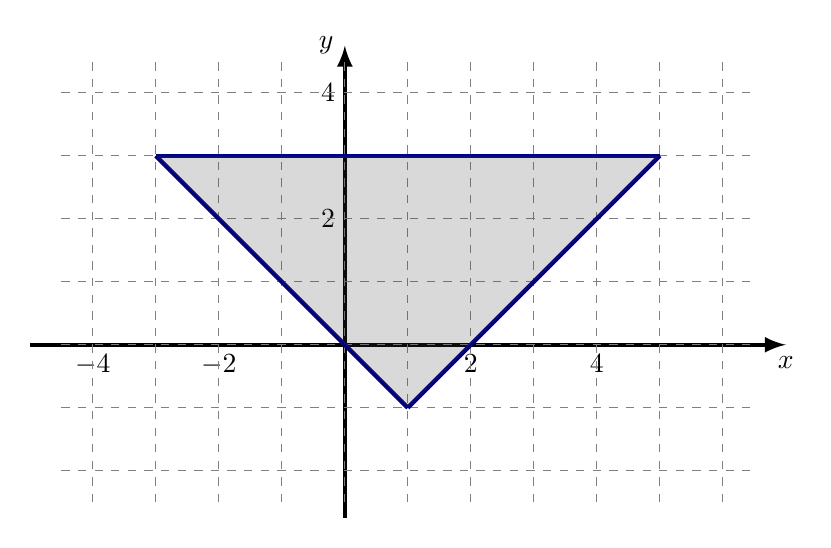
\begin{tikzpicture}[scale=0.8]
        \draw[ultra thick,->,>=latex] (-5,0)--(7,0) node[below] {$x$};
        \draw[ultra thick,->,>=latex] (0,-2.75)--(0,4.75) node[left] {$y$};
        \draw (-4,0) node[below] {$-4$};          
        \draw (-2,0) node[below] {$-2$};          
        \draw (2,0) node[below] {$2$};          
        \draw (4,0) node[below] {$4$};          
        \draw (0,2) node[left] {$2$};        
        \draw (0,4) node[left] {$4$};
        \draw[help lines,gray,thin,dashed] (-4.5, -2.5) grid (6.5, 4.5);
        \draw[domain=-3:1,ultra thick,DarkBlue,samples=4] plot ({\x},{-\x });
        \draw[domain=1:5,ultra thick,DarkBlue,samples=4] plot ({\x},{\x-2});
        \draw[ultra thick,-,DarkBlue,>=latex] (-3,3)--(5,3);
        \draw[fill=gray!50!black, opacity=0.2] (-3,3) -- (1,-1) -- (5,3);                
    \end{tikzpicture}
    \end{center}      
    The region is also
    \begin{align}
            -y \le x \le y+2, \quad -1 \le y \le 3
    \end{align}
    Thus
    \begin{align}
        V = \int_{-1}^3\int_{-y}^{y+2} f(x,y) \, dx\, dy
    \end{align}
    }
   \else
   \fi
\fi 

% REGION OUTSIDE CIRCLE
\ifnum \Version=7
    \part $\displaystyle \int_{0}^{4} \int_{\sqrt{16-x^2}}^{4}  dy \, dx = \int_{a}^{b} \int_{c}^{d}  d x\,  d y$, where 
    $a=\framebox{\strut\hspace{1cm}}$, $b=\framebox{\strut\hspace{1cm}}$, $c=\framebox{\strut\hspace{2cm}}$, and $d=\framebox{\strut\hspace{2cm}}$.    

    \ifnum \Solutions=1 
    {\color{DarkBlue}
    We are given that 
    \begin{align}
        0 \le x \le 4, \quad \sqrt{16 - x^2} \le y \le 4
    \end{align}
    The region is also
    \begin{align}
        0 \le y \le 4, \quad \sqrt{16 - y^2} \le x \le 4
    \end{align}
    Thus
    \begin{align}
        \int_{0}^{4} \int_{\sqrt{16-x^2}}^{4}  d y \, d x = \int_0^4\int_{\sqrt{16 - y^2}}^4 \, dx \, dy
    \end{align}
    So
    \begin{align}
        a &= 0 \\
        b &= 4 \\
        c &= \sqrt{16-y^2} \\
        d &= 4
    \end{align}    
    }
   \else

   \fi
\fi 







% 15.2
% WEIRD REGION, TWO INTEGRALS TO ONE, MAYBE A HARD QUESTION? 
\ifnum \Version=8
    \part $\displaystyle \int_{1}^{5} \int_{0}^{\sqrt{x-1}} f(x,y) d y \, d x + \int_{5}^{7} \int_{0}^{7-x} f(x,y) d y \, d x = \int_{a}^{b} \int_{c}^{d} f(x,y) \, d x\,  d y$, where 
    $a=\framebox{\strut\hspace{1.5cm}}$, $b=\framebox{\strut\hspace{1.5cm}}$, $c=\framebox{\strut\hspace{4cm}}$, and $d=\framebox{\strut\hspace{4cm}}$.    

    \ifnum \Solutions=1 
    {\color{DarkBlue}
    We are given two regions: 
    \begin{align}
        R_1: &\ 1 \le x \le 5, \quad 0 \le y \le \sqrt{x-1} \\
        R_2: &\ 5 \le x \le 7, \quad 0 \le y \le \sqrt{7-x}
    \end{align}
    The region is also
    \begin{align}
            y^2+1 \le x \le 7-x, \quad 0 \le y \le 2
    \end{align}
    Thus
    \begin{align}
        a &= 0 \\
        b &= 2 \\
        c &= y^2+1 \\
        d &= 7-x
    \end{align}
    }
   \else
   \fi
\fi 




% 15.2
% REGION ABOVE A PARABOLA
\ifnum \Version=9
    \part Let $\displaystyle A = \iint_R  d y \, d x = \int_{a}^{b} \int_{c}^{d}  d x\,  d y$, where $R=\{(x,y) \in \mathbb R^2 \, | \,0 \le x \le 2, \ x^2+1 \le y \le 5 \} $. Then 
    $a=\framebox{\strut\hspace{1.5cm}}$, $b=\framebox{\strut\hspace{1.5cm}}$, $c=\framebox{\strut\hspace{2cm}}$, and $d=\framebox{\strut\hspace{3cm}}$.    

    \ifnum \Solutions=1 
    {\color{DarkBlue}
    We are given that 
    \begin{align}
        0 \le x \le 2, \quad x^2+1 \le y \le 5
    \end{align}
    The region is also
    \begin{align}
        0 \le x \le \sqrt {y-1}, \quad 1 \le y \le 5
    \end{align}
    Thus
    \begin{align}
        \int_{0}^{2} \int_{x^2+1}^{1}  d y \, d x = \int_1^5\int_0^{\sqrt{y-1}} \, dx\, dy
    \end{align}
    So
    \begin{align}
        a &= 1\\
        b &= 5 \\
        c &= 0 \\
        d &= \sqrt{y-1}
    \end{align}    
    }
   \else

   \fi
\fi 

    % SECTIONS 14.3 TO 14.4

% SECTIONS 14.3 TO 14.4
\ifnum \Version=1
% THOMAS 14.3
% SLOPE OF TANGENT LINE

\part Consider the surface $f(x,y) = x^3+y^2$ and the point $P(10,3)$. The slope of the tangent line to the surface at $P$ and is in the plane $x=10$ is $\framebox{\strut\hspace{1cm}}$. The slope of the tangent line to the surface at $P$ and is in the plane $y=3$ is $\framebox{\strut\hspace{1cm}}$.

\ifnum \Solutions=1 {\color{DarkBlue} \textit{Solutions:} the tangent line for any $y$ and constant $x$ has slope
$$\frac{\partial f}{\partial y} = \frac{\partial}{\partial y}\left( x^3+y^2 \right) = 2y$$
At the point $(10,3)$ the tangent line has slope $2\cdot 3 = 6$. Likewise the tangent line for any $x$ and constant $y$ has slope
$$\frac{\partial f}{\partial x} = \frac{\partial}{\partial x}\left( x^3+y^2 \right) = 3x^2$$
At the point $(10,3)$ the tangent line has slope $3\cdot 10^2 = 300$. 
}
\else
  
\fi
\fi


\ifnum \Version=2
% THOMAS 14.4
% IMPLICIT

\part Compute the value of $\displaystyle \DZDY$ at the point $P(1,3,2)$ if $x + z^2y = 19$ defines $z$ as a function of the two independent variables $x$ and $y$ and the partial derivative exists. $\displaystyle \DZDY$ at $P$ is $\framebox{\strut\hspace{1cm}}$.

\ifnum \Solutions=1 {\color{DarkBlue} Implicit differentiation:
\begin{align}
    x + z^2y &= 19 \\
    \DDY \left( x + z^2y \right) &= \DDY \, 19 \\
    0 + 2z\DZDY y + z^2 &= 0 
\end{align}
At the point $(1,3,2)$ this is
\begin{align}
     2(2)\DZDY (3) + (2)^2 &= 0 \\
     12\DZDY + 4 &= 0 \\
     \DZDY &= - 4/12
\end{align}
}
\else
\fi
\fi

\ifnum \Version=3
% THOMAS 14.4
% CHAIN

\part The partial derivatives of a function $f(x,y)$ on the curve $x(t) = t$, $y(t) = t^2-4t$ are $f_x=-t$, $f_y=1$. Then along this curve, the extreme values of $f(x,y)$ occur when $t = \framebox{\strut\hspace{2cm}}$.

\ifnum \Solutions=1 {\color{DarkBlue} \vspace{6pt}\textit{Answer:} $t =4$ \\[12pt] \textit{Solutions:} by the chain rule: $$\frac{df}{dt}=\frac{df}{dx}\frac{dx}{dt}+ \frac{df}{dy}\frac{dy}{dt} = (-t) (1) + (1)(2t-4) = t - 4$$
The maximum values occur when $df/dt=0$. Thus 
$$\frac{df}{dt} = t-4 =0 \quad \Rightarrow \quad t = 4$$
}
\else
  
\fi
\fi



\ifnum \Version=4
% THOMAS 14.4
% CHAIN

\part An object travels along a path on a surface $z=z(x,y)$.  At time $t=t_0$ it is known that
	\[ \DZDX=-4, \quad \DZDY=2, \quad \dfrac{dx}{dt}=3, \quad \dfrac{dy}{dt}=8. \]
	The rate of change of the height $z$ of the object with respect to $t$ at $t=t_0$ is $\framebox{\strut\hspace{1cm}}$.

\ifnum \Solutions=1 {\color{DarkBlue} \vspace{6pt}\textit{Answer:} $t =4$ \\[12pt] \textit{Solutions:} by the chain rule: $$\frac{dz}{dt}=\DZDX\frac{dx}{dt}+ \DZDY\frac{dy}{dt} = (-4)(3) + (2)(8) = -12 + 16 = 4$$
}
\else
  
\fi
\fi





% SECTIONS 14.3 TO 14.4
\ifnum \Version=5
% THOMAS 14.3
% INTERPRET DERIVATIVE

\part Suppose $f(x,y)$ is the surface given by $f(x,y) = x^2y + 4$. The slope of the line tangent to this surface that is in the plane $y=2$ and is at the point $(3,2)$ is $\framebox{\strut\hspace{2cm}}$.

\ifnum \Solutions=1 {\color{DarkBlue} \vspace{6pt}\textit{Answer:} $12$ \\[12pt] \textit{Solutions:} the tangent line for any $x$ and constant $y$ has slope
$$\frac{\partial f}{\partial x} = \frac{\partial}{\partial x}\left( x^2y + 4 \right) = 2xy$$
At the point $(3,2)$ the tangent line has slope $2\cdot 3 \cdot 2 = 12$. 
}
\else
  
\fi
\fi


% SECTIONS 14.3 TO 14.4
\ifnum \Version=6
% THOMAS 14.3
% INTERPRET DERIVATIVE

\part Suppose $f(x,y)$ is the surface given by $f(x,y) = x^2y + 4$. The slope of the line tangent to this surface that is in the plane $y=2$ and is at the point $(3,2)$ is $\framebox{\strut\hspace{2cm}}$.

\ifnum \Solutions=1 {\color{DarkBlue} \vspace{6pt}\textit{Answer:} $12$ \\[12pt] \textit{Solutions:} the tangent line for any $x$ and constant $y$ has slope
$$\frac{\partial f}{\partial x} = \frac{\partial}{\partial x}\left( 2x^2 + 3y - 4 \right) = 4x$$
At the point $(3,-4)$ the tangent line has slope $4\cdot 3 = 12$. 
}
\else
  
\fi
\fi




% SECTIONS 14.3 TO 14.4
\ifnum \Version=7
% THOMAS 14.3
% SLOPE OF TANGENT LINE

\part Consider the surface $f(x,y) = x^2+xy-y^2$ and the point $P(4,1)$. The slope of the tangent line to the surface at $P$ and is in the plane $x=4$ is $\framebox{\strut\hspace{1cm}}$. The slope of the tangent line to the surface at $P$ and is in the plane $y=1$ is $\framebox{\strut\hspace{1cm}}$.

\ifnum \Solutions=1 {\color{DarkBlue} \textit{Solutions:} there are two parts to this question. 
\begin{itemize}
    \item The tangent line for any $y$ and constant $x$ has slope
    $$\frac{\partial f}{\partial y} = \frac{\partial}{\partial y}\left( x^2+xy-y^2 \right) = x-2y$$
    At the point $(4,1)$ the tangent line has slope $4-2\cdot1 = 2$. 
    \item Likewise the tangent line for any $x$ and constant $y$ has slope
    $$\frac{\partial f}{\partial x} = \frac{\partial}{\partial x}\left( x^2+xy-y^2 \right) = 2x+y$$
    At the point $(4,1)$ the tangent line has slope $2\cdot4 + 1 = 9$. 
\end{itemize}
}
\else
  
\fi
\fi


\ifnum \Version=8
% THOMAS 14.4
% CHAIN

\part An object travels along a path on a surface $z=z(x,y)$.  At time $t=t_0$ it is known that
	\[ \DZDX=3, \quad \dfrac{dx}{dt}=10, \quad \DZDY=6, \quad \dfrac{dy}{dt}=2. \]
	The rate of change of the height $z$ of the object with respect to $t$ at $t=t_0$ is $\framebox{\strut\hspace{1cm}}$.

\ifnum \Solutions=1 {\color{DarkBlue} \textit{Solutions:} by the chain rule: $$\frac{dz}{dt}=\DZDX\frac{dx}{dt}+ \DZDY\frac{dy}{dt} = (3)(10) + (6)(2) = 30 + 12 = 42$$
}
\else
  
\fi
\fi


\ifnum \Version=9
% THOMAS 14.4
% CHAIN

\part An object travels along a path on a surface $z=z(x,y)$.  At time $t=t_0$ it is known that
	\[ \DZDX=2, \quad \dfrac{dx}{dt}=5, \quad \DZDY=10, \quad \dfrac{dy}{dt}=7. \]
	The rate of change of the height $z$ of the object with respect to $t$ at $t=t_0$ is $\framebox{\strut\hspace{1cm}}$.

\ifnum \Solutions=1 {\color{DarkBlue} \textit{Solutions:} by the chain rule: $$\frac{dz}{dt}=\DZDX\frac{dx}{dt}+ \DZDY\frac{dy}{dt} = (2)(5) + (10)(7) = 10 + 70 = 80$$
}
\else
  
\fi
\fi

\ifnum \Version=10
% THOMAS 14.4
% IMPLICIT

\part Compute the values of $\displaystyle \DZDX$ and $\displaystyle \DZDY$ at the point $P(-1,2,1)$ if $y + xz^2 = 1$ defines $z$ as a function of the two independent variables $x$ and $y$ and the partial derivative exists. $\displaystyle \DZDX$ at $P$ is $\framebox{\strut\hspace{1cm}}$, and $\displaystyle \DZDY$ at $P$ is $\framebox{\strut\hspace{1cm}}$. 

\ifnum \Solutions=1 {\color{DarkBlue} This question has two parts. 

\begin{itemize}
    \item Implicit differentiation with $\DDX$:
    \begin{align}
        y+xz^2 &= 1 \\
        \DDX \left( y+xz^2 \right) &= 0 \\
        0 + z^2 + 2xz\DZDX&= 0 
    \end{align}
    At the point $(-1,2,1)$ this is
    \begin{align}
         1^2 + 2\cdot (-1) \cdot 1 \cdot\DZDX &= 0 \\
         1  - 2 z_x &= 0 \\
         z_x &=  1/2
    \end{align}
    \item Implicit differentiation with $\DDY$:
    \begin{align}
        y+xz^2 &= 1 \\
        \DDY \left( y+xz^2 \right) &= 0 \\
        1 + 2xz\DZDY&= 0 
    \end{align}
    At the point $(-1,2,1)$ this is
    \begin{align}
         1 + 2(-1)(1)\DZDY &= 0 \\
         -2\DZDY &= -1 \\
         \DZDY &= 1/2
    \end{align}
\end{itemize}
}
\else
\fi
\fi



\ifnum \Version=11
% THOMAS 14.4
% IMPLICIT

\part Compute the values of $\displaystyle \DZDX$ and $\displaystyle \DZDY$ at the point $P(-1,2,1)$ if $y + xz^2 = 1$ defines $z$ as a function of the two independent variables $x$ and $y$ and the partial derivative exists. $\displaystyle \DZDX$ at $P$ is $\framebox{\strut\hspace{1cm}}$, and $\displaystyle \DZDY$ at $P$ is $\framebox{\strut\hspace{1cm}}$. 

\ifnum \Solutions=1 {\color{DarkBlue} This question has two parts. 

\begin{itemize}
    \item Implicit differentiation with $\DDX$:
    \begin{align}
        y+xz^2 &= 1 \\
        \DDX \left( y+xz^2 \right) &= 0 \\
        0 + z^2 + 2xz\DZDX&= 0 
    \end{align}
    At the point $(-1,2,1)$ this is
    \begin{align}
         1^2 + 2\cdot (-1) \cdot 1 \cdot\DZDX &= 0 \\
         1  - 2 z_x &= 0 \\
         z_x &=  1/2
    \end{align}
    \item Implicit differentiation with $\DDY$:
    \begin{align}
        y+xz^2 &= 1 \\
        \DDY \left( y+xz^2 \right) &= 0 \\
        1 + 2xz\DZDY&= 0 
    \end{align}
    At the point $(-1,2,1)$ this is
    \begin{align}
         1 + 2(-1)(1)\DZDY &= 0 \\
         -2\DZDY &= -1 \\
         \DZDY &= 1/2
    \end{align}
\end{itemize}
}
\else
\fi
\fi
    %12.6 

\ifnum \Version=1 
\part Identify the surface $x^2-y+2z^2 = 4$ by type (cone, paraboloid, etc.). \framebox{\strut\hspace{3cm}}.

\ifnum \Solutions=1 {\color{DarkBlue} \textit{Answer:} elliptical paraboloid \\[12pt] \textit{Solutions:} The curve can be expressed as $y=x^2+2z^2 -4$. In the plane $x=0$ the curve is a parabola $y=2z^2-4$. In the plane $z=0$ the curve is a parabola $y=x^2-4$. Both parabolas open over the $y$-axis. It is more accurate to refer to this shape as an elliptical paraboloid, but we'll be nice and give full credit for writing paraboloid. We do this because many people refer to $y = x^2$ and $y=2x^2$ as parabolas. So, for us, it isn't necessary to indicate that the surface is an \textbf{elliptical} paraboloid. It is sufficient to refer to this surface as a paraboloid. But be careful: a hyperbolic paraboloid is not a paraboloid! Do not refer to hyperbolic paraboloid as a paraboloid. 
} 
\else
  
\fi
\fi


\ifnum \Version=2
\part Identify the surface $-x^2+y^2+4z^2 = 0$ by type (cone, paraboloid, etc.). \framebox{\strut\hspace{3cm}}.

\ifnum \Solutions=1 {\color{DarkBlue} \textit{Answer:} elliptical cone \\[12pt] \textit{Solutions:} The curve can be expressed as $x^2=y^2+4z^2$. In the plane $x=k$ for constant $k$, the curve is an ellipse with equation $y^2+4z^2=k$. The surface intersects the plane $z=0$ along two straight lines $x=\pm y$, and likewise the plane $y=0$ along the lines $z = \pm 4z$. \textit{Note that it isn't necessary to indicate that the surface is an \textbf{elliptical} cone. It is sufficient to refer to this surface as a cone. There is no such thing as a hyperbolic cone, in this course.}
} 
\else
  
\fi
\fi



\ifnum \Version=3
\part Identify the surface $x^2+2z^2 = 16+4y-y^2$ by type (cone, ellipsoid, etc.). \framebox{\strut\hspace{4.0cm}}.

\ifnum \Solutions=1 {\color{DarkBlue} \textit{Answer:} ellipsoid\\[12pt] \textit{Solutions:} Rearrange and complete the square. 
\begin{align*}
    x^2+2z^2 &= 16+4y-y^2\\
   16&= y^2-4y+ x^2+2z^2 \\
   16&= y^2-4y+4-4 + x^2+2z^2 \\
   16&= (y-2)^2 -4 + x^2+2z^2 \\
   20&= (y-2)^2 + x^2+2z^2 
\end{align*}
Not a sphere because coefficient in front of squared terms not all the same. Surface is an ellipsoid. We can refer to spheres as ellipsoids (because a sphere is a special case of an ellipsoid), but we can't refer to an ellipsoid as a sphere unless the ellipsoid is a shpere. 
} 
\else
  
\fi
\fi






\ifnum \Version=4
\part Identify the surface $y+z^2 = 1-x^2$ by type (cone, ellipsoid, etc.). \framebox{\strut\hspace{4.6cm}}.

\ifnum \Solutions=1 {\color{DarkBlue} \textit{Answer:} paraboloid. The vertex of the paraboloid is at the point $(0,1,0)$. It is ok to call this an elliptical paraboloid, because a paraboloid is a type of elliptical paraboloid. On the other hand, it is not correct to call this a hyperbolic paraboloid, because that is a very different surface! 
} 
\else
  
\fi
\fi


\ifnum \Version=5
\part Identify the surface $x-y^2-2y=4z^2 $ by type (cone, ellipsoid, etc.). \framebox{\strut\hspace{4cm}}.

\ifnum \Solutions=1 {\color{DarkBlue} \textit{Answer:} paraboloid \\[12pt] \textit{Solutions:} In the plane $x=k$ for constant $k$, the curves are ellipses.But in the plane $y=0$, we have a parabola $x = 4z^2$. So we can call this surface a paraboloid or elliptical paraboloid. It is more accurate to refer to this shape as an elliptical paraboloid, but we'll be nice and give full credit for writing paraboloid. We do this because many people refer to $y = x^2$ and $y=2x^2$ as parabolas. So, for us, it isn't necessary to indicate that the surface is an \textbf{elliptical} paraboloid. It is sufficient to refer to this surface as a paraboloid. But be careful: a hyperbolic paraboloid is not a paraboloid! Do not refer to hyperbolic paraboloid as a paraboloid.
} 
\else
  
\fi
\fi


\ifnum \Version=6
\part Identify the surface $x-y^2+z^2 = 0$ by type (cone, ellipsoid, etc.). \framebox{\strut\hspace{4.6cm}}.

\ifnum \Solutions=1 {\color{DarkBlue} \textit{Answer:} saddle, or hyperbolic paraboloid. It would not be correct to refer to this shape as a paraboloid. A paraboloid is a very different surface. 
} 
\else
  
\fi
\fi

\ifnum \Version=7
\part Identify the surface $x^2-y^2+z = 0$ by type (cone, ellipsoid, etc.). \framebox{\strut\hspace{4.6cm}}.

\ifnum \Solutions=1 {\color{DarkBlue} \textit{Answer:} saddle, or hyperbolic paraboloid. It would not be correct to refer to this shape as a paraboloid. A paraboloid is a very different surface. 
} 
\else
\fi
\fi

\ifnum \Version=8
\part Identify the surface $-x^2-y^2+z = 0$ by type (cone, ellipsoid, etc.). \framebox{\strut\hspace{4.6cm}}.

\ifnum \Solutions=1 {\color{DarkBlue} \textit{Answer:} elliptical paraboloid. 
} 
\else
  
\fi
\fi


\ifnum \Version=9
\part Identify the surface $-x^2+y-2z^2 = 0$ by type (cone, ellipsoid, etc.). \framebox{\strut\hspace{4.6cm}}.

\ifnum \Solutions=1 {\color{DarkBlue} \textit{Answer:} paraboloid, or elliptical paraboloid. 
} 
\else
  
\fi
\fi


\ifnum \Version=10
\part Identify the surface $x-5y^2-2z^2 = 0$ by type (cone, ellipsoid, etc.). \framebox{\strut\hspace{4.6cm}}.

\ifnum \Solutions=1 {\color{DarkBlue} \textit{Answer:} paraboloid, or elliptical paraboloid. 
} 
\else
  
\fi
\fi
    % TRIPLE INTEGRALS IN RECTANGULAR
% THOMAS 15.5

% VERBATIM THOMAS - CAN EASILY CREATE MORE VERSIONS IF NEEDED
\ifnum \Version=1

    \part $\displaystyle \int_{-1}^1 \int_{x^2}^1 \int_0^{1-y} dz \, dy \, dx = \int_a^b \int_c^d \int_h^k  \, dx \, dz \,dy$, where 
    $a=\framebox{\strut\hspace{1.0cm}}$, $b=\framebox{\strut\hspace{1.0cm}}$, $c=\framebox{\strut\hspace{1.4cm}}$, $d=\framebox{\strut\hspace{1.4cm}}$, $h=\framebox{\strut\hspace{2.0cm}}$,
    $k=\framebox{\strut\hspace{2.0cm}}$.

    \ifnum \Solutions=1 
    {\color{DarkBlue} We are given
    \begin{align}
        -1 \le \, &x \le 1 \\
        x^2 \le \, &y \le 1 \\
        0 \le \, &z \le 1-y 
    \end{align}
    Thus,
    \begin{align}
        0 \le \, &y \le 1 \\
        0 \le \, &z \le 1-y \\
        -\sqrt{y} \le \, &x \le \sqrt{y}
    \end{align}
    The triple integral becomes
    \begin{align}
        \int_{-1}^1 \int_{x^2}^1 \int_0^{1-y} dz \, dy \, dx = \int_a^b \int_c^d \int_h^k  \, dx \, dz \,dy
    \end{align}
    }
   \else

   \fi
    
\fi


\ifnum \Version=2

    \part The volume of the tetrahedron cut from the first octant by the plane $6x+3y+z=6$ is $\displaystyle \int_a^b \int_c^d \int_0^k  \, dz \, dy\,dx$, where $a=\framebox{\strut\hspace{1.2cm}}$, $b=\framebox{\strut\hspace{1.2cm}}$, $c=\framebox{\strut\hspace{2.2cm}}$, $d=\framebox{\strut\hspace{2.2cm}}$, and $k=\framebox{\strut\hspace{2.6cm}}$.
    
    \ifnum \Solutions=1 
    {\color{DarkBlue} \textit{Solutions:}
    When $y=z=0$, the plane cuts the $x$-axis at $x=1$. So every point in the solid has $x$-coordinates between $x=0$ and $x=1$. 
    When $z=0$, the plane cuts the $xy$-plane along the line \begin{align}
        6x+3y+0 &= 6 \\
        y &= 2-2x
    \end{align}
    So every point in the solid has $y$-coordinates between $y=0$ and $y=2-2x$. 
    The solid is bounded below by the $xy-$plane and above by the plane $6x+3y+z=6$, or 
    \begin{align}
        0 \le z \le 6-6x-3y
    \end{align}
    The triple integral is
    $$\displaystyle \int_{0}^{1}\int_{0}^{2-2x} \int_0^{6-6x-3y} \, dz \, dy \, dx$$
    }
    \else

    \fi
    
\fi







\ifnum \Version=3
% VERBATUM 2022

    \part $\displaystyle \int_{0}^{1}\int_{\sqrt x}^{1} \int_0^{1-y} f(x,y,z) \, dz \, dy \, dx = \int_a^b \int_c^d \int_0^k f(x,y,z) \, dz \, dx\,dy$, where $a=\framebox{\strut\hspace{1.2cm}}$, $b=\framebox{\strut\hspace{1.2cm}}$, $c=\framebox{\strut\hspace{1.2cm}}$, $d=\framebox{\strut\hspace{1.2cm}}$, $k=\framebox{\strut\hspace{1.2cm}}$.

    % stewart 13.7 # 31

    \ifnum \Solutions=1 
    {\color{DarkBlue} \textit{Solutions:}
    $$\displaystyle \int_{0}^{1}\int_{\sqrt x}^{1} \int_0^{1-y} f(x,y,z) \, dz \, dy \, dx = \int_0^1 \int_0^{y^2} \int_0^{1-y} f(x,y,z) \, dz \, dx \,dy$$
    }
    \else

    \fi
    
\fi


\ifnum \Version=4

    \part $\displaystyle \int_{0}^{1}\int_{\sqrt x}^{1} \int_0^{1-y} f(x,y,z) \, dz \, dy \, dx = \int_a^b \int_c^d \int_0^k f(x,y,z) \, dx \, dz\,dy$, where $a=\framebox{\strut\hspace{1.6cm}}$, \\ $b=\framebox{\strut\hspace{1.6cm}}$, $c=\framebox{\strut\hspace{1.4cm}}$, $d=\framebox{\strut\hspace{1.4cm}}$, $k=\framebox{\strut\hspace{1.4cm}}$.

    % stewart 13.7 # 31

    \ifnum \Solutions=1 
    {\color{DarkBlue} \textit{Solutions:}
    $$\displaystyle \int_{0}^{1}\int_{\sqrt x}^{1} \int_0^{1-y} f(x,y,z) \, dz \, dy \, dx = \int_0^1 \int_0^{1-y} \int_0^{y^2} f(x,y,z) \, dx \, dz \,dy$$
    }
    \else

    \fi
    
\fi

\ifnum \Version=5

    \part The volume of the tetrahedron cut from the first octant by the plane $4x+y+z=12$ is $\displaystyle \int_0^a \int_0^b \int_c^d  \, dy \, dz\,dx$, where $a=\framebox{\strut\hspace{2.2cm}}$, $b=\framebox{\strut\hspace{2.2cm}}$, $c=\framebox{\strut\hspace{2.2cm}}$, and $d=\framebox{\strut\hspace{3cm}}$.
    
    \ifnum \Solutions=1 
    {\color{DarkBlue} \textit{Solutions:}
    Consider each of the three variables separately. 
    \begin{itemize}
        \item When $y=z=0$, the plane cuts the $x$-axis at $x=12/4=3$. So every point in the solid has $x$-coordinates between $x=0$ and $x=3$. 
        \item When $y=0$, the plane cuts the $xz$-plane along the line \begin{align}
        4x+z+0 &= 12 \\
        z &= 12 -4x
    \end{align}
    So every point in the solid has $z$-coordinates between $z=0$ and $z=12-4x$. 
    \item The solid is bounded by the $xz-$plane and to the right by the plane $4x+y+z=12$, or 
    \begin{align}
        0 \le y \le 12 -4x-z
    \end{align}
    \end{itemize}
    The region is the set 
    \begin{align}
        V = \{(x,y,z) \in \mathbb R^3 \, | \, 0\le x\le 3, 0 \le z \le 12 - 4x, 0 \le y \le 12 - 4x - z \}
    \end{align}
    The triple integral is
    $$\displaystyle \int_{0}^{3}\int_{0}^{12-4x} \int_0^{12-4x-z} \, dy \, dz \, dx$$
    Thus:
    \begin{align}
        a&=3 \\
        b&= 12-4x \\
        c &= 0 \\
        d &= 12-4x-z
    \end{align}
    }
    \else

    \fi
    
\fi




% THOMAS 
% 12e, 15.5 #21
% HALF CIRCULAR CYLINDER BOUNDED ABOVE BY SURFACE
\ifnum \Version=6

    \part $E$ is a solid that lies above the $xy-$plane, and is bounded by $x^2+y^2=1$, and also the plane $z=-y$. The volume of region $E$ is $\displaystyle V = \int_{A}^B \int_{C}^D \int_0^K dz \, dy \, dx$, where 
    $A=\framebox{\strut\hspace{1.0cm}}$, $B=\framebox{\strut\hspace{1.0cm}}$, $C=\framebox{\strut\hspace{3cm}}$, $D=\framebox{\strut\hspace{3cm}}$,    $K=\framebox{\strut\hspace{3cm}}$.

    \ifnum \Solutions=1 
    {\color{DarkBlue} We consider each of the variables individually, starting with the outermost integral and working our way to the innermost integral. 
    \begin{itemize}
        \item \textbf{Outermost integral}: For the region to lie in the cylinder $x^2+y^2=1$ we must have that 
        \begin{align}
            -1 \le \, &x \le 1 
        \end{align}
        \item \textbf{Middle integral}: because the region is bounded above by $z = -y$ and below by $z=0$, the $y-$values must be negative. The portion of the cylinder that corresponds to negative $y-$values are the lower portion of the unit circle in the $xy-$plane shown below.
        \begin{center}     
        \begin{tikzpicture}[scale=1.25]
            \begin{axis}[
            axis lines = middle, very thick,
            xlabel = {$x$},
            ylabel = {$y$},
            xmin=-3, xmax=3,
            ymin=-3, ymax=3,
            xtick={-2,-1,0,1,2},
            xticklabels={-2,-1,0,1,2},  
            ytick={-2,-1,0,1,2},
            yticklabels={-2,-1,0,1,2},    
            ]
            % Plot 1
            \addplot [name path = A,-,domain = -1:1, ultra thick,DarkBlue, samples = 100] {-sqrt(1-x^2} node [right=2pt] {};
            \node (l) at (1.5,-1) {$x^2+y^2 = 1$};
            \addplot [name path = B,-,domain = -1:1, ultra thick,DarkBlue, samples = 4] {0} node [very near end, right=4pt] {}; 
            % Fill area between paths
            \addplot [black!30, opacity=0.2] fill between [of = A and B, soft clip={domain=-1:1}];
            \end{axis}
        \end{tikzpicture}    
        \end{center}         
        \item \textbf{Innermost Integral}: for any given $x$ and $z$ in the solid, points in the solid will have a $z-$coordinate between $0$ and $z=-y$. 
        \begin{align}
            0 \le z \le -y
        \end{align}
    \end{itemize}

    The triple integral is
    $$\displaystyle \iiint_E dV = \int_{-1}^{1}\int_{-\sqrt{1-x^2}}^{0} \int_0^{-y} \, dy \, dz \, dx$$
    Therefore,
    \begin{align}
        A &= -1 \\
        B &= 1 \\
        C & = -\sqrt{1-x^2}\\
        D &= 0 \\
        K &= - y
    \end{align}

    }
   \else

   \fi
    
\fi





% TETRAHEDRON IN FIRST QUADRANT
\ifnum \Version=7

    \part The volume of the tetrahedron cut from the first octant by the plane $6x+y+3z=12$ is $\displaystyle \int_A^B \int_0^D \int_0^K   \, dy\, dz \,dx$, where $A=\framebox{\strut\hspace{1.2cm}}$, $B=\framebox{\strut\hspace{1.2cm}}$, $D=\framebox{\strut\hspace{3cm}}$, and $K=\framebox{\strut\hspace{3cm}}$.
    
    \ifnum \Solutions=1 
    {\color{DarkBlue} \textit{Solutions:}
    We consider each of the variables individually, starting with the outermost integral and working our way to the innermost integral. 
    \begin{itemize}
        \item \textbf{Outermost integral}: When $y=z=0$, the plane cuts the $x$-axis at the point where $$6x + 0 + 3\cdot 0 = 12$$ Or where $x=2$. So every point in the solid has $x$-coordinates between $x=0$ and $x=2$. 
        \item \textbf{Middle integral}: When $y=0$, the plane cuts the $xz$-plane along the line 
        \begin{align}
            6x+3\cdot 0 + 3z &= 12 \\
            z &= 4-2x
        \end{align}
        So every point in the solid has $z$-coordinates between $z=0$ and $z=4-2x$. 
        \item \textbf{Innermost Integral}: for any given $x$ and $z$ in the solid, points in the solid will have a $y-$coordinate between $0$ and $y=12-3z-6x$. 
        \begin{align}
            0 \le y \le 12 - 6x-3z
        \end{align}
    \end{itemize}

    The triple integral is
    $$\displaystyle \int_{0}^{2}\int_{0}^{4-2x} \int_0^{12-6x-3z} \, dy \, dz \, dx$$
    Therefore,
    \begin{align}
        A &= 0 \\
        B &= 2 \\
        D & = 4-2x\\
        K &= 12-6x-3z
    \end{align}
    }
    \else

    \fi
    
\fi



% THOMAS 
% 12e, 15.5 #21
% HALF CIRCULAR CYLINDER BOUNDED ABOVE BY SURFACE
\ifnum \Version=8

    \part Region $E$ lies above the $xy-$plane, and is bounded by $x^2+y^2=1$ and the plane $z=-x$. The volume of region $E$ is $\displaystyle V = \int_{A}^B \int_{C}^D \int_0^K dz \, dx \, dy$, where 
    $A=\framebox{\strut\hspace{1.0cm}}$, $B=\framebox{\strut\hspace{1.0cm}}$, $C=\framebox{\strut\hspace{3cm}}$, $D=\framebox{\strut\hspace{3cm}}$,    $K=\framebox{\strut\hspace{3cm}}$.

    \ifnum \Solutions=1 
    {\color{DarkBlue} We consider each of the variables individually, starting with the outermost integral and working our way to the innermost integral. 
    \begin{itemize}
        \item \textbf{Outermost integral}: For the region to lie in the cylinder $x^2+y^2=1$ we must have that 
        \begin{align}
            -1 \le \, y \le 1 
        \end{align}
        \item \textbf{Middle integral}: because the region is bounded above by $z = -x$ and below by $z=0$, the $z-$coordinates within $E$ must be positive and the $x-$coordinates within $D$ must be negative. The portion of the cylinder that corresponds to negative $x-$values are the \textbf{left portion} of the unit circle in the $xy-$plane shown below. 
        \begin{center}     
        \begin{tikzpicture}[scale=1.25]
            \begin{axis}[
            axis lines = middle, very thick,
            xlabel = {$x$},
            ylabel = {$y$},
            xmin=-3, xmax=3,
            ymin=-3, ymax=3,
            xtick={-2,-1,0,1,2},
            xticklabels={-2,-1,0,1,2},  
            ytick={-2,-1,0,1,2},
            yticklabels={-2,-1,0,1,2},    
            ]
            % Plot 1
            \addplot [name path = A,-,domain = -1:0, ultra thick,DarkBlue, samples = 25] {-sqrt(1-x^2} node [right=2pt] {};
            \node (l) at (-1.65,0.8) {$x^2+y^2 = 1$};
            % Plot 2
            \addplot [name path = B,-,domain = -1:0, ultra thick,DarkBlue, samples = 25] {+sqrt(1-x^2} node [right=2pt] {};
            % Fill area between paths
            \addplot [black!30, opacity=0.2] fill between [of = A and B, soft clip={domain=-1:0}];
            \end{axis}
        \end{tikzpicture}    
        \end{center}         
        The $x-$coordinates are 
        \begin{align}
            -\sqrt{1-y^2} \le x \le \sqrt{1-y^2}
        \end{align}
        \item \textbf{Innermost Integral}: for any given $x$ and $y$ in the solid, points in the solid will have a $z-$coordinate between $0$ and $z=-x$. 
        \begin{align}
            0 \le z \le -x
        \end{align}
    \end{itemize}

    The triple integral is
    $$\displaystyle \iiint_E dV =\int_{-1}^{1}\int_{-\sqrt{1-y^2}}^{\sqrt{1-y^2}} \int_0^{-x} \, dz \, dx \, dy$$
    Therefore,
    \begin{align}
        A &= -1 \\
        B &= 1 \\
        C & = -\sqrt{1-y^2}\\
        D &= \sqrt{1-y^2} \\
        K &= - x
    \end{align}

    }
   \else

   \fi
    
\fi





% THOMAS 
% 12e, 15.5 #21
% PARBOLA IN TWO QUADRANTS AND BELOW Z = 10 - Y
\ifnum \Version=9

    \part The solid $E$ lies above the $xy-$plane, below the surface $z=10-y$, and is bounded by the surface $y=4-x^2$ and the plane $y=0$. The volume of region $E$ is $\displaystyle V = \int_{A}^B \int_{C}^D \int_0^K dz \, dy \, dx$, where 
    $A=\framebox{\strut\hspace{1.0cm}}$, $B=\framebox{\strut\hspace{1.0cm}}$, $C=\framebox{\strut\hspace{3cm}}$, $D=\framebox{\strut\hspace{3cm}}$,    $K=\framebox{\strut\hspace{3cm}}$.

    \ifnum \Solutions=1 
    {\color{DarkBlue} Because the region is bounded above by $z = 10-y$, below by $z=0$, and on the sides by $y=0$ and $y=4-x^2$, the $y-$coordinates within $E$ must be positive. The projection of all the points, in the solid, onto the $xy-$plane are shown below. 
        \begin{center}  
        \begin{tikzpicture}[scale=1.25]
            \begin{axis}[
            axis lines = middle, very thick,
            xlabel = {$x$},
            ylabel = {$y$},
            xmin=-5, xmax=5.75,
            ymin=-3, ymax=5.75,
            xtick={-4,-2,0,2,4},
            xticklabels={-4,-2,0,2,4},
            ytick={-2,0,2,4},
            yticklabels={-2,0,2,4}        
            ]
            % Plot 1
            \addplot [name path = A,-,domain = -2:2, line width=0.8mm,DarkBlue,samples = 30] {4-x^2} ;
            % Vertical line
            \addplot[name path = B,line width=0.8mm,samples=4, smooth,domain=0:6,DarkBlue, name path=three] coordinates {(-2,0)(2,0)};
            % Fill area between paths
            \addplot [black!30, opacity=0.2] fill between [of = A and B, soft clip={domain=-2:2}];
            \end{axis}
        \end{tikzpicture}    
        \end{center}   
        We consider each of the variables individually, starting with the outermost integral and working our way to the innermost integral. 
    \begin{itemize}
        \item \textbf{Outermost integral}: For the region to lie in the cylinder $y=4-x^2$, and also have positive $y-$coordinates, we must have that 
        \begin{align}
            -2 \le \, x \le 2
        \end{align}
        \item \textbf{Middle integral}: 
        For any given $x$, the $y-$values range from $x=0$ to $y=4-x^2$. The $y-$coordinates are 
        \begin{align}
            0 \le y \le 4-x^2
        \end{align}
        \item \textbf{Innermost Integral}: for any given $x$ and $y$ in the solid, points in the solid will have a $z-$coordinate between $0$ and $z=10-y$. 
        \begin{align}
            0 \le z \le 10-y
        \end{align}
    \end{itemize}
    The triple integral is
    $$\displaystyle \int_{-2}^{2}\int_{0}^{4-x^2} \int_0^{10-y} \, dz \, dy \, dx$$
    Therefore,
    \begin{align}
        A &= -2 \\
        B &= 2 \\
        C &= 0\\
        D &= 4-x^2 \\
        K &= 10-y
    \end{align}

    }
   \else

   \fi
    
\fi
    % APPLICATIONS or CYLINDRICAL or SPHERICAL (THOMAS 15.6 OR 15.7)


\ifnum \Version=1
% SHORT SPHERICAL AND CYLINDRICAL EXERCISE
% VERBATUM FROM SPRING 2022 QUIZ
% hand written solution only
\part Point $P$ has rectangular (Cartesian) coordinates $(x,y,z) = (0,-3,4)$ in $\mathbb R^3$. In cylindrical coordinates, the point is $(r,\theta,z)$, and in spherical coordinates the point is $(\rho, \phi, \theta)$. Where $r=\framebox{\strut\hspace{1cm}}$, $\theta=\framebox{\strut\hspace{1cm}}$, $z=\framebox{\strut\hspace{1cm}}$, $\rho=\framebox{\strut\hspace{1.5cm}}$, and $\phi=\framebox{\strut\hspace{3cm}}$. 

    \ifnum \Solutions=1 {\color{DarkBlue} \textit{Solutions:} To convert to cylindrical we can use the equation $r^2 = x^2 + y^2$. 
    \begin{align}
        r^2 &= x^2 + y^2 = 0^2 + (-3)^2 = 9 \ \Rightarrow \ r = 3 
    \end{align}
    To determine $\theta$ we notice that $P$ lies on the $y-$axis and has a negative $y$ value. So $\theta = 3\pi/2$.
    $$\displaystyle (r,\theta,z) = (3,\frac{3\pi}2,4)$$
    In spherical, we can start by obtaining $\rho$. 
    \begin{align}
        \rho^2 &= x^2+y^2+z^2\\
        \rho^2 &= 0^2 + (-3)^2 + 4^2 = 25 \\
        \rho &= 5 
    \end{align}
    To obtain $\phi$ we can use the equation that relates $y$ to spherical. Using the expression for $y$, and the values that we already have for $y$, $\rho$ and $\theta$:
    \begin{align}
        y &= \rho \sin\phi \sin\theta \\
        -3 &= 5\sin\phi \sin(3\pi/2) \\
        3 &= 5\sin\phi \\
        \sin\phi &= 3/5 \\
        \phi &= \arcsin (3/5)
    \end{align}
    Our coordinates in spherical are
    \begin{align}
        \rho &= 5\\
        \phi &= \arcsin (3/5)\\
        \theta &= \frac{3\pi}2  
    \end{align}
    Note the following.
    \begin{itemize}
        \item Note that we could also obtain $\phi$ using a right-angle triangle in the $yz-$plane. 
        \item Other similar approaches can lead to other equivalent expressions for $\phi$, such as $\phi = \arctan(3/4)$.
        \item Our particular textbook uses the convention $(\rho, \phi, \theta)$, not $(\rho, \theta,\phi)$.
    \end{itemize}
    } 
    \else
      
    \fi
    
\fi

% 15.6
% BASED ON  THOMAS, 15.6 #3
% GOOD PROBLEM FOR #4, EASY
\ifnum \Version=2
    \part A thin plate of density $\delta(x,y)=2$ is bounded by $y=x-1$ and $y=5-x^2$. The plate has mass $M$, and the $y-$coordinate of the center of mass is $\bar y = M_x/M$, where $M_x = \int_a^b \int_c^d f(x,y) \, dy \, dx$,  and $b=\framebox{\strut\hspace{1.0cm}}$, $c=\framebox{\strut\hspace{2cm}}$, $d=\framebox{\strut\hspace{2cm}}$, and $f(x,y) = \framebox{\strut\hspace{2cm}}$. 

    \ifnum \Solutions=1
    {\color{DarkBlue}
    The region is bounded by 
    $$x-1 \le y \le 5-x^2$$
    The given curves intersect when 
    \begin{align}
        x-1 &= 5-x^2 \\
        0 &= x^2 +x -6 \\
        &= (x+3)(x-2)
    \end{align}
    Thus
    \begin{align}
        \bar y &= \frac{M_x}M = \frac1M \int_{-3}^{2}\int_{x-1}^{5-x^2} 2y \, dy \, dx
    \end{align} 
    The density of the plate is $\delta = 2$. Thus
    \begin{align}
        a &= -3 \\
        b &= 2 \\
        c&= x-1 \\
        d&= 5-x^2 \\
        f(x,y) &= \delta y = 2y
    \end{align}
    }
   \else
   \fi
    
\fi






% 15.6
% BASED ON  THOMAS, 15.6 Example 2
% GOOD PROBLEM FOR #3, EASY
\ifnum \Version=3
    \part $R$ is the region in the $xy-$plane bounded by $y=4x$ and the curve $y=x^2$. Then $R$ has area $M$, and the $x-$coordinate of the centroid is $\bar x = M_y/M$, where $M_y = \int_a^b \int_c^d f(x,y) \, dy \, dx$,  and $a=\framebox{\strut\hspace{1.0cm}}$, $b=\framebox{\strut\hspace{1.0cm}}$, $c=\framebox{\strut\hspace{2cm}}$, $d=\framebox{\strut\hspace{2cm}}$, and $f(x,y) = \framebox{\strut\hspace{2cm}}$. 
    
    \ifnum \Solutions=1 
    {\color{DarkBlue}
    The region is bounded by 
    $$x^2 \le y \le 4x$$
    The curves $y=x^2$ and $y=4x$ intersect at $x=0$ and $x=4$. 
    Thus
    \begin{align}
        \bar x &= \frac1M \int_{0}^{4}\int_{x^2}^{4x} x \, dy \, dx
    \end{align} 
    Thus,
    \begin{align}
        a &= 0 \\
        b &= 4 \\
        c&= x^2 \\
        d&= 4x \\
        f(x,y) &= x
    \end{align}
    }
    \newpage
   \else

   \fi
    
\fi



% 15.6
% BASED ON  THOMAS, 15.6 #3
% GOOD PROBLEM FOR #4, EASY
\ifnum \Version=4
    \part A thin plate with density $\delta=4$ is bounded in the $xy-$plane by $x=2-y$ and $x=y^2$. The plate has mass $M$, and the $y-$coordinate of the center of mass is $\bar y = M_x/M$, where $M_x = \int_a^b \int_c^d f(x,y) \, dx \, dy$,  and $a=\framebox{\strut\hspace{0.8cm}}$, $b=\framebox{\strut\hspace{0.8cm}}$, $c=\framebox{\strut\hspace{1.0cm}}$, $d=\framebox{\strut\hspace{1.0cm}}$, $f(x,y) = \framebox{\strut\hspace{1.0cm}}$. 
    
    \ifnum \Solutions=1 
    {\color{DarkBlue}
    The region is bounded by 
    $$y^2 \le x \le 2-y$$
    The given curves intersect when 
    \begin{align}
        y^2 &= 2-y \\
        0 &= y^2 +y -2 \\
        &= (y-1)(y+2)
    \end{align}
    Thus
    \begin{align}
        \bar y &= \frac{M_x}M = \frac1M \int_{-2}^{1}\int_{y^2}^{2-y} 4y \, dx \, dy
    \end{align} 
    Thus
    \begin{align}
        a &= -2 \\
        b &= 1 \\
        c&= y^2 \\
        d&= 2-y \\
        f(x,y) &= \delta y = 4y
    \end{align}
    }
   \else

   \fi
    
\fi



\ifnum \Version=5
% SHORT SPHERICAL AND CYLINDRICAL EXERCISE
\part Point $P$ has rectangular (Cartesian) coordinates $(x,y,z) = (2,2,1)$ in $\mathbb R^3$. In cylindrical coordinates, the point is $(r,\theta,z)$, and in spherical coordinates the point is $(\rho, \phi, \theta)$. Where $r=\framebox{\strut\hspace{1cm}}$, $\theta=\framebox{\strut\hspace{2cm}}$, $z=\framebox{\strut\hspace{1cm}}$, $\rho=\framebox{\strut\hspace{2cm}}$, and $\phi=\framebox{\strut\hspace{3cm}}$. 

    \ifnum \Solutions=1 {\color{DarkBlue} \textit{Solutions:} To convert to cylindrical we can use the equation $r^2 = x^2 + y^2$. 
    \begin{align}
        r^2 &= x^2 + y^2 = 2^2 + 2^2 = 8 \ \Rightarrow \ r = 2\sqrt2
    \end{align}
    To determine $\theta$ we can use $\tan\theta = y/x$. 
    \begin{align}
        \tan \theta &= \frac{y}{x} = \frac{2}{2} = 1  \\
        \theta &= \arctan 1 = \pi/4
    \end{align} 
    The point in cylindrical is: 
    \begin{align}
        (r,\theta,z) &= (2\sqrt2,\pi/4,1) \\
        r &= 2\sqrt2 \\
        \theta &= \pi/4 \\
        z &= 1
    \end{align}
    In spherical, we can start by obtaining $\rho$. 
    \begin{align}
        \rho^2 &= x^2+y^2+z^2\\
        \rho^2 &= 2^2 + 2^2 + 1^2 = 9 \\
        \rho &= 3
    \end{align}
    To obtain $\phi$ we can use the equation that relates $y$ to spherical. Using the expression for $y$, and the values that we already have for $y$, $\rho$ and $\theta$:
    \begin{align}
        y &= \rho \sin\phi \sin\theta \\
        2 &= 3\sin\phi \sin(\pi/4) \\
        \sin\phi &= \frac{2}{3 \sin(\pi/4)}  = \frac{2\sqrt2}{3}\\
        \phi &= \arcsin (2\sqrt2/3)
    \end{align}
    Our coordinates in spherical are
    \begin{align}
        \rho &= 3\\
        \phi &= \arcsin (2\sqrt2/3)\\
        \theta &= \pi/4
    \end{align}
    Note the following.
    \begin{itemize}
        \item Note that we could also obtain $\phi$ using the equation $x = \rho \sin\phi \cos\theta$ but we would obtain the same answer with just as much work. 
        \item We can, for this exercise, leave un-evaluated trig functions in the answer, because the question didn't specify that you should simplify your answer as much as possible. So it would be ok to leave your answer for $\theta$ as $\arctan 1$ or $\tan^{-1} 1$. 
        \item Our particular textbook uses the convention $(\rho, \phi, \theta)$, not $(\rho, \theta,\phi)$.
    \end{itemize}
    } 
    \else
      
    \fi
    
\fi



% 15.6
% BASED ON  THOMAS, 15.6 #3
% EASY? NOT SURE? 
\ifnum \Version=6
    \part A thin plate with density $\delta=12$ is bounded in the $xy-$plane by $y=x-2$ and $x=y^2$. The plate has mass $M$, and the $y-$coordinate of the center of mass is $\bar y = M_x/M$, where $M_x = \int_a^b \int_c^d f(x,y) \, dx \, dy$,  and $a=\framebox{\strut\hspace{1.5cm}}$, $b=\framebox{\strut\hspace{1.5cm}}$, $c=\framebox{\strut\hspace{3.0cm}}$, $d=\framebox{\strut\hspace{3.0cm}}$, and $f(x,y) = \framebox{\strut\hspace{2.0cm}}$. 
    
    \ifnum \Solutions=1 
    {\color{DarkBlue}
    The region is bounded by 
    $$y^2 \le x \le y+2$$
    The given curves intersect when 
    \begin{align}
        y^2 &= y+2 \\
        0 &= y^2 - y -2 \\
        &= (y-2)(y+1)
    \end{align}
    The curves intersect at $y=-1,2$. Using $x=y^2$, the intersection points are $(1,-1)$ and $(4,2)$. The region is shown below. 
    \begin{center}  
        \begin{tikzpicture}[scale=1.25]
            \begin{axis}[
            axis lines = middle, very thick,
            xlabel = {$x$},
            ylabel = {$y$},
            xmin=-5, xmax=5.75,
            ymin=-3.5, ymax=5.75,
            xtick={-4,-2,0,2,4},
            xticklabels={-4,-2,0,2,4},
            ytick={-2,0,2,4},
            yticklabels={-2,0,2,4}        
            ]
            % Curves
            \addplot [name path = A,-,domain = 0:5, line width=0.8mm,DarkBlue,samples = 30] {sqrt(x)} ;
            \addplot [name path = B,-,domain = 0:5, line width=0.8mm,DarkBlue,samples = 30] {-sqrt(x)} ;
            \addplot [name path = C, line width=0.8mm, samples=4, smooth,domain=0:5, DarkBlue] coordinates {(-1,-3)(5,3)};
            % Fill area between paths
            \addplot [black!30, opacity=0.2] fill between [of = A and B, soft clip={domain=0:1}];
            \addplot [black!30, opacity=0.2] fill between [of = A and C, soft clip={domain=1:4}];
            \end{axis}
        \end{tikzpicture}    
    \end{center}   
        
    Thus
    \begin{align}
        \bar y &= \frac{M_x}M = \frac1M \int_{-1}^{2}\int_{y^2}^{y+2} 12y \, dx \, dy
    \end{align} 
    Thus
    \begin{align}
        a &= -1 \\
        b &= 2 \\
        c&= y^2 \\
        d&= y+2 \\
        f(x,y) &= \delta y = 12y
    \end{align}
    }
   \else

   \fi
    
\fi

\ifnum \Version=7
% SHORT SPHERICAL AND CYLINDRICAL EXERCISE
\part Point $P$ has rectangular (Cartesian) coordinates $(x,y,z) = (-6,0,8)$ in $\mathbb R^3$. In cylindrical coordinates, the point is $(r,\theta,z)$, and in spherical coordinates the point is $(\rho, \phi, \theta)$. Where $r=\framebox{\strut\hspace{1cm}}$, $\theta=\framebox{\strut\hspace{2cm}}$, $z=\framebox{\strut\hspace{1cm}}$, $\rho=\framebox{\strut\hspace{2cm}}$, and $\phi=\framebox{\strut\hspace{3cm}}$. 

    \ifnum \Solutions=1 {\color{DarkBlue} \textit{Solutions:} To convert to cylindrical we can use the equation $r^2 = x^2 + y^2$. 
    \begin{align}
        r^2 &= x^2 + y^2 = (-6)^2 + 0^2 = 36 \ \Rightarrow \ r = 6
    \end{align}
    To determine $\theta$ we can use $\tan\theta = y/x$. 
    \begin{align}
        \tan \theta &= \frac{y}{x} = \frac{0}{-6} = 0  \\
        \theta &= \arctan 0 
    \end{align} 
    The point in cylindrical is: 
    \begin{align}
        (r,\theta,z) &= (6,\pi,8) \\
        r &= 6 \\
        \theta &= \pi \\
        z &= 8
    \end{align}
    In spherical, we can start by obtaining $\rho$. 
    \begin{align}
        \rho^2 &= x^2+y^2+z^2\\
        \rho^2 &= (-6)^2 + 0^2 + 8^2 = 36+64 = 100 \\
        \rho &= 10
    \end{align}
    To obtain $\phi$ we can use the equation that relates $x$ to spherical. Using the expression for $x$, and the values that we already have for $x$, $\rho$ and $\theta$:
    \begin{align}
        x &= \rho \sin\phi \cos\theta \\
        -6 &= 10\sin\phi \cos(\pi) \\
        \sin\phi &= \frac{-6}{10 \cos(\pi)}  = \frac{6}{10}\\
        \phi &= \arcsin (6/10)
    \end{align}
    Our coordinates in spherical are
    \begin{align}
        \rho &= 10\\
        \phi &= \arcsin (6/10)\\
        \theta &= \pi
    \end{align}
    Note the following.
    \begin{itemize}
        \item We can, for this exercise, leave un-evaluated trig functions in the answer, because the question didn't specify that you should simplify your answer as much as possible. So it would be ok to leave your answer for $\theta$ as $\arctan 0$ or $\tan^{-1} 0$. 
        \item Our particular textbook uses the convention $(\rho, \phi, \theta)$, not $(\rho, \theta,\phi)$.
    \end{itemize}
    } 
    \else
      
    \fi
    
\fi





\ifnum \Version=8
% SHORT SPHERICAL AND CYLINDRICAL EXERCISE
\part Point $P$ has rectangular (Cartesian) coordinates $(x,y,z) = (4,4,7)$ in $\mathbb R^3$. In cylindrical coordinates, the point is $(r,\theta,z)$, and in spherical coordinates the point is $(\rho, \phi, \theta)$. Where $r=\framebox{\strut\hspace{1cm}}$, $\theta=\framebox{\strut\hspace{2cm}}$, $z=\framebox{\strut\hspace{1cm}}$, $\rho=\framebox{\strut\hspace{2cm}}$, and $\phi=\framebox{\strut\hspace{3cm}}$. 

    \ifnum \Solutions=1 {\color{DarkBlue} \textit{Solutions:} To convert to cylindrical we can use the equation $r^2 = x^2 + y^2$. 
    \begin{align}
        r^2 &= x^2 + y^2 = (4)^2 + 4^2 = 32 \ \Rightarrow \ r = \sqrt{32} = 4\sqrt2
    \end{align}
    It isn't necesssary to simplify to $4\sqrt2$. Then to determine $\theta$ we can use $\tan\theta = y/x$. 
    \begin{align}
        \tan \theta &= \frac{y}{x} = \frac{4}{4} = 1  \\
        \theta &= \arctan \pi/4
    \end{align} 
    The point in cylindrical is: 
    \begin{align}
        (r,\theta,z) &= (4\sqrt2,\pi/4,7) \\
        r &= 4\sqrt2 \\
        \theta &= \pi/4 \\
        z &= 7
    \end{align}
    In spherical, we can start by obtaining $\rho$. 
    \begin{align}
        \rho^2 &= x^2+y^2+z^2\\
        \rho^2 &= (4)^2 + 4^2 + 7^2 = 16+16+49 = 32+49 = 81 \\
        \rho &= 9
    \end{align}
    To obtain $\phi$ we can use the equation that relates $x$ to spherical. Using the expression for $x$, and the values that we already have for $x$, $\rho$ and $\theta$:
    \begin{align}
        x &= \rho \sin\phi \cos\theta \\
        4 &= 9\sin\phi \cos(\pi/4) \\
        \sin\phi &= \frac{4}{9 \cos(\pi/4)}  = \frac{4\sqrt2}{9}\\
        \phi &= \arcsin \left(\frac{4\sqrt2}{9}\right)
    \end{align}
    Note for $\phi$ we can also use:
    \begin{align}
        y &= \rho \sin\phi \sin\theta \\
        4 &= 9\sin\phi \sin(\pi/4) \\
        \sin\phi &= \frac{4}{9 \sin(\pi/4)}  = \frac{4\sqrt2}{9}\\
        \phi &= \arcsin \left(\frac{4\sqrt2}{9}\right)
    \end{align}    
    And we can also use:
    \begin{align}
        z &= \rho \cos\phi  \\
        7 &= 9\cos\phi  \\
        \sin\phi &= \frac{4}{9 \sin(\pi/4)}  = \frac{4\sqrt2}{9}\\
        \phi &= \arccos \left(\frac{7}{9}\right)
    \end{align}      
    Our coordinates in spherical are
    \begin{align}
        \rho &= 9\\
        \phi &= \arcsin \left(\frac{4\sqrt2}{9}\right), \ \textbf{or} \ \phi = \arccos(7/9)\\
        \theta &= \pi/4
    \end{align}
    Note the following.
    \begin{itemize}
        \item We can, for this exercise, leave un-evaluated trig functions in the answer, because the question didn't specify that you should simplify your answer as much as possible. So it would be ok to leave your answer for $\theta$ as $\arctan 1$ or $\tan^{-1} 1$. 
        \item Our particular textbook uses the convention $(\rho, \phi, \theta)$, not $(\rho, \theta,\phi)$.
    \end{itemize}
    } 
    \else
      
    \fi
    
\fi





% 15.6
% CENTROID Y-COORDINATE PARABOLA AND LINE
\ifnum \Version=9
    \part A thin plate with density $\delta=12$ is bounded in the $xy-$plane by $y=3-x^2$ and $y=1-x$. The plate has mass $M$. The $y-$coordinate of the centroid is $\bar y = M_x/M$, where $\displaystyle M_x = \int_A^B \int_C^D f(x,y) \, dy \, dx$,  and $A=\framebox{\strut\hspace{1cm}}$, $B=\framebox{\strut\hspace{1cm}}$, $C=\framebox{\strut\hspace{3cm}}$, $D=\framebox{\strut\hspace{3cm}}$, and $f(x,y) = \framebox{\strut\hspace{3cm}}$. 
    
    \ifnum \Solutions=1 
    {\color{DarkBlue}
    The region is bounded by 
    $$1-x \le y \le 3-x^2$$
    The given curves intersect when 
    \begin{align}
        1-x &= 3-x^2\\
        0 &= x^2-x-2 \\
        &= (x-2)(x+1)
    \end{align}
    The curves intersect at $x=-1,2$. Using $y=1-x$, the intersection points are $(-1,2)$ and $(2,-1)$. The region is shown below. 
    \begin{center}  
        \begin{tikzpicture}[scale=1.25]
            \begin{axis}[
            axis lines = middle, very thick,
            xlabel = {$x$},
            ylabel = {$y$},
            xmin=-5, xmax=5.75,
            ymin=-3.5, ymax=5.75,
            xtick={-4,-2,0,2,4},
            xticklabels={-4,-2,0,2,4},
            ytick={-2,0,2,4},
            yticklabels={-2,0,2,4}        
            ]
            % Curves
            \addplot [name path = A,-,domain = -2.2:2.5, line width=0.8mm,DarkBlue,samples = 30] {3-x^2} ;
            \addplot [name path = C,-,domain = -2.2:2.5, line width=0.8mm,DarkBlue,samples = 4] {1-x} ;
            % Fill area between paths
            \addplot [black!30, opacity=0.2] fill between [of = A and C, soft clip={domain=-1:2}];
            \end{axis}
        \end{tikzpicture}    
    \end{center}   
        
    Thus
    \begin{align}
        \bar y &= \frac{M_x}M = \frac1M \int_{-1}^{2}\int_{1-x}^{3-x^2} 12y \, dy \, dx
    \end{align} 
    Thus
    \begin{align}
        A &= -1 \\
        B &= 2 \\
        C&= 1-x \\
        D&= 3-x^2 \\
        f(x,y) &= \delta y = 12y
    \end{align}
    }
   \else

   \fi
    
\fi
   
    % 15.8 JACOBIAN OR CHANGE OF VARIABLE



\ifnum \Version=1
    \part Consider the transform $u=x+y$ and $v=y-2x$. Then $x = u/3 - v/3$, and $ y = 2u/3+v/3$. Using the transform, $\displaystyle \int_0^1\int_0^{1-x} \sqrt{x+y}( y-2x) \, dy \,dx =  \int_a^b \int_c^d g(u,v) \, dv \, du$,  where $a=\framebox{\strut\hspace{1cm}}$, $b=\framebox{\strut\hspace{1cm}}$, $c=\framebox{\strut\hspace{2cm}}$, $d=\framebox{\strut\hspace{2cm}}$, and $g(u,v) = \framebox{\strut\hspace{2cm}}$. Hint: the Jacobian of the transform is $1/3$. 

    \ifnum \Solutions=1 
    {\color{DarkBlue} 
    We need to transform the limits of integration, and we need to transform $\sqrt{x+y}(y-2x) \, dy \,dx$. 
    \textbf{Transform the Integrand and Differentials}\\
    The integrand becomes
    \begin{align}
        \sqrt{x+y} (y -2x) = \sqrt{u}\, v = v\sqrt u
    \end{align}
    Therefore, 
    \begin{align}
        \sqrt{x+y} (y -2x) \, dy\,dx = \sqrt{u}\, v = v\sqrt u \, \left| \frac{1}{3} \right| \, dv \, du = \frac{v\sqrt u}{3} \, dv \, du
    \end{align}    
    So $$g(u,v) = \frac{v\sqrt u}{3}$$
    \textbf{Limits of integration}\\ 
    The region in the $xy-$plane, $R$, is the set 
    $$R = \{(x,y) \in \mathbb R \, | \, 0 \le x \le 1, \ 0 \le y \le 1-x \}$$
    The triangular region is shown below. 
    \begin{center}     
    \begin{tikzpicture}[scale=1]
        \begin{axis}[
        axis lines = middle, very thick,
        xlabel = {$x$},
        ylabel = {$y$},
        xmin=-0.8, xmax=1.75,
        ymin=-0.8, ymax=1.75,
        xtick={0,1},
        xticklabels={0,1},  
        ytick={0,1},
        yticklabels={0,1},    
        ]
        % Plot 1
        \addplot [name path = A,
        -,
        domain = 0:1, ultra thick,DarkBlue,
        samples = 100] {1-x} 
        node [right=2pt] {};
        \node[text=DarkBlue] (t) at (1,.75) {$y=1-x$};
        \node[text=DarkBlue] (left) at (-0.35,.5) {$x=0$};
        \node[text=DarkBlue] (bottom) at (0.5,-.25) {$y=0$};
        \node (l) at (.25,.25) {$R$};
        \addplot[ultra thick, samples=50, smooth,domain=0:1,DarkBlue] coordinates {(0,0)(0,1)};        
        \addplot [name path = B,
        -,
        domain = 0:1, ultra thick,DarkBlue,
        samples = 100] {0} 
        node [very near end, right=4pt] {}; 
        % Fill area between paths
        \addplot [black!30, opacity=0.2] fill between [of = A and B, soft clip={domain=0:1}];
        \end{axis}
    \end{tikzpicture}    
    \end{center}     
    To determine the boundaries in the $uv-$plane we transform each of the boundaries individually. 
    \begin{itemize}
        \item \textbf{Left boundary}: using $x = u/3 - v/3$, the line $x=0$ becomes $u=v$. 
        \item \textbf{Lower boundary}: using $y = 2u/3+v/3$, the line $y=0$ becomes $v=-2u$. 
        \item \textbf{Upper boundary}: line $y=1-x$ becomes 
        \begin{align}
            y&= 1- x \\
            2u/3+v/3 &= 1 - (u/3 - v/3) \\
            2u+v &= 3- u +v \\
            u &= 1
        \end{align}
    \end{itemize}
    The region in the $uv-$plane, $G$, is 
    $$G = \{(u,v) \in \mathbb R^2 \, | \, 0 \le u \le 1, \ -2u \le v \le u \}$$

    \textbf{Putting Everything Together}\\
    Therefore, 
    \begin{align}
        a & = 0 \\
        b &= 1 \\
        c &= -2u \\
        d &= u \\
        g &= \frac{v\sqrt u}{3}
    \end{align}
    
    \textbf{Additional Notes}\\
    Two additional notes about this question. 
    \begin{itemize}
        \item Note that we did not need to obtain $x$ and $y$ in terms of $u,v$, because we were given $x(u,v)$ and $y(u,v)$. But if we needed to express $x$ and $y$ in terms of $u$ and $v$, we could use the expressions for $u$ and $v$ as an augmented matrix and row reduce. 
    \begin{align}
        \begin{pmatrix} 1 & 1 & u \\-2 & 1 & v\end{pmatrix} 
        \sim \begin{pmatrix} 1 & 1 & u \\0 & 3 & v + 2u\end{pmatrix} 
        \sim \begin{pmatrix} 1 & 1 & u \\0 & 1 & 2u/3 + v/3\end{pmatrix} 
        \sim \begin{pmatrix} 1 & 0 & u/3-v/3 \\0 & 1 & 2u/3 + v/3\end{pmatrix} 
    \end{align}
    Thus
    \begin{align}
        x &= u/3 - v/3\\
        y &= 2u/3+v/3
    \end{align}
    \item Also it isn't necessary to sketch the region in the $uv-$plane, but it can help when determining the limits of integration in the transformed integral. The region is shown below. 
    \begin{center}     
    \begin{tikzpicture}[scale=1]
        \begin{axis}[
        axis lines = middle, very thick,
        xlabel = {$u$},
        ylabel = {$v$},
        xmin=-0.1, xmax=2.75,
        ymin=-2.75, ymax=1.75,
        xtick={0,1,2},
        xticklabels={0,1,2},  
        ytick={-2,-1,0,1},
        yticklabels={-2,-1,0,1},    
        ]
        % Plot 1
        \addplot [name path = A,
        -,
        domain = 0:1, ultra thick,DarkBlue,
        samples = 100] {x} 
        node [right=2pt] {};
        \node[text=DarkBlue] (t) at (.6,.95) {$u=v$};
        \node[text=DarkBlue] (left) at (1.3,.5) {$u=1$};
        \node[text=DarkBlue] (bottom) at (0.4,-1.75) {$v=-2u$};
        \node (l) at (.65,-.5) {$G$};
        \addplot[ultra thick, samples=50, smooth,domain=0:1,DarkBlue] coordinates {(1,-2)(1,1)};    
        % Plot 2
        \addplot [name path = B, -,
        domain = 0:1, ultra thick,DarkBlue, samples = 100] {-2*x} node [very near end, right=4pt] {}; 
        % Fill area between paths
        \addplot [black!30, opacity=0.2] fill between [of = A and B, soft clip={domain=0:1}];
        \end{axis}
    \end{tikzpicture}    
    \end{center}     
    \end{itemize}
    
    
    }
   \else

   \fi
\fi 






\ifnum \Version=2
    \part Consider the transform $u=x+y$ and $v=x-y$. Then $x = (u+v)/2$, and $y = (u-v)/2$. Using this transform, $\displaystyle \int_0^2\int_{-y}^{y} f(x,y) \, dx \,dy =  \int_a^b \int_c^d g(u,v) \, dv \, du$,  where $a=\framebox{\strut\hspace{1cm}}$, $b=\framebox{\strut\hspace{1cm}}$, $c=\framebox{\strut\hspace{2cm}}$, $d=\framebox{\strut\hspace{2cm}}$. 

    \ifnum \Solutions=1 
    {\color{DarkBlue} 
    We only need to transform the limits of integration. The region in the $xy-$plane, $R$, is the set 
    $$R = \{(x,y) \in \mathbb R \ | \ 0 \le y \le 2, \ -y \le x \le y \}$$
    The triangular region is shown below. 
    \begin{center}     
    \begin{tikzpicture}[scale=1]
        \begin{axis}[
        axis lines = middle, very thick,
        xlabel = {$x$},
        ylabel = {$y$},
        xmin=-2.75, xmax=2.75,
        ymin=-0.8, ymax=2.75,
        xtick={-2,-1,0,1,2},
        xticklabels={-2,-1,0,1,2},  
        ytick={0,1,2},
        yticklabels={0,1,2},    
        ]
        % Plot Right
        \addplot [name path = R, -, domain = 0:2, ultra thick,DarkBlue, samples = 100] {x} node [right=2pt] {};
        % Plot Left
        \addplot [name path = L, -, domain = -2:0, ultra thick,DarkBlue, samples = 100] {-x} node [right=2pt] {};
        \node[text=DarkBlue] (right) at (1.35,.75) {$y=x$};
        \node[text=DarkBlue] (left) at (-1.45,.75) {$y=-x$};
        \node[text=DarkBlue] (bottom) at (0.75,2.25) {$y=2$};
        \node (l) at (0.35,1.35) {$R$};
        \addplot [name path = T,-, domain = -2:2, ultra thick,DarkBlue,samples = 100] {2} node [very near end, right=4pt] {}; 
        % Fill area between paths
        \addplot [black!30, opacity=0.2] fill between [of = L and T, soft clip={domain=-2:0}];
        \addplot [black!30, opacity=0.2] fill between [of = R and T, soft clip={domain=0:+2}];
        \end{axis}
    \end{tikzpicture}    
    \end{center}     
    To determine the boundaries in the $uv-$plane we transform each of the boundaries individually. 
    \begin{itemize}
        \item \textbf{Left boundary}: using $u=x+y$, the line $y=-x$ becomes $u=0$. 
        \item \textbf{Right boundary}: using $v=x-y$, the line $y=x$ becomes $v=0$. 
        \item \textbf{Top boundary}: using $y=(u-v)/2$, the line $y=2$ becomes 
        \begin{align}
            2 &= (u-v)/2 \\
            4 &= u - v \\
            v &= u - 4
        \end{align}
    \end{itemize}
    The region in the $uv-$plane, $G$, is 
    $$G = \{(u,v) \in \mathbb R^2 \, | \, 0 \le u \le 4, \ u-4 \le v \le 0 \}$$
    \textbf{Putting Everything Together}\\
    Therefore, 
    \begin{align}
        a & = 0 \\
        b &= 4 \\
        c &= u-4 \\
        d &= 0 
    \end{align}
    
    \textbf{Additional Notes}\\
    Two additional notes about this question. 
    \begin{itemize}
        \item Note that we did not need to obtain $x$ and $y$ in terms of $u,v$, because we were given $x(u,v)$ and $y(u,v)$. But if we needed to express $x$ and $y$ in terms of $u$ and $v$, we could use the expressions for $u$ and $v$ as an augmented matrix and row reduce. 
    \begin{align}
        \begin{pmatrix} 1 & 1 & u \\1 & -1 & v\end{pmatrix} 
        \sim \begin{pmatrix} 1 & 1 & u \\0 & -2 & v - u\end{pmatrix} 
        \sim \begin{pmatrix} 1 & 1 & u \\0 & 1 & (u - v)/2\end{pmatrix} 
        \sim \begin{pmatrix} 1 & 0 & (u + v)/2 \\0 & 1 & (u - v)/2\end{pmatrix} 
    \end{align}
    Thus
    \begin{align}
        x &=  (u + v)/2\\
        y &= (u - v)/2
    \end{align}
    \item Also it isn't necessary to sketch the region in the $uv-$plane, but it can help when determining the limits of integration in the transformed integral. The region is shown below. 
    \begin{center}     
    \begin{tikzpicture}[scale=1]
        \begin{axis}[
        axis lines = middle, very thick,
        xlabel = {$u$},
        ylabel = {$v$},
        xmin=-1.1, xmax=4.75,
        ymin=-4.75, ymax=2.75,
        xtick={0,2,4},
        xticklabels={0,2,4},  
        ytick={-4,-2,0,2},
        yticklabels={-4,-2,0,2},    
        ]
        % Plot 1
        \addplot [name path = B, -,domain = 0:4, ultra thick,DarkBlue, samples = 100] {x-4} node [right=2pt] {};
        \node[text=DarkBlue] (t) at (2,-3) {$v = u-4$};
        \node[text=DarkBlue] (left) at (1.3,.5) {$v=0$};
        \node[text=DarkBlue] (bottom) at (-0.6,-1) {$u=0$};
        \node (l) at (.85,-1) {$G$};
        \addplot[ultra thick, samples=50, smooth,domain=0:1,DarkBlue] coordinates {(0,-4)(0,0)};    
        % Plot 2
        \addplot [name path = T, -,
        domain = 0:4, ultra thick,DarkBlue, samples = 100] {0} node [very near end, right=4pt] {}; 
        % Fill area between paths
        \addplot [black!30, opacity=0.2] fill between [of = B and T, soft clip={domain=0:4}];
        \end{axis}
    \end{tikzpicture}    
    \end{center}     
    \end{itemize}
    
    
    }
   \else

   \fi
\fi 




\ifnum \Version=3
    \part Consider the transform $u=x-1$ and $v=x+y/2$. Then $x = u+1$, and $y = 2v-2u-2$. Using this information, $\displaystyle \int_0^2\int_{4-2x}^{8-2x} \sqrt{x+y/2} \, dy \,dx =  \int_a^b \int_c^d g(u,v) \, dv \, du$,  where $a=\framebox{\strut\hspace{1cm}}$, $b=\framebox{\strut\hspace{1cm}}$, $c=\framebox{\strut\hspace{2cm}}$, $d=\framebox{\strut\hspace{2cm}}$, and the Jacobian of the transform is $J(u,v) = \framebox{\strut\hspace{2cm}}$. 

    \ifnum \Solutions=1 
    {\color{DarkBlue} 
    We need to transform the limits of integration and determine the Jacobian. The Jacobian is
    \begin{align}
        J(u,v) 
        & = \begin{vmatrix} \DXDU & \DXDV \\[8pt] \DYDU & \DYDV \end{vmatrix} 
        = \begin{vmatrix} 1 & 0 \\ -2 & 2 \end{vmatrix} 
        = 2
    \end{align}   
    To work out the limits of integration, we can start by determining the boundaries of the region in the $xy-$plane. The region in the $xy-$plane, $R$, is the set 
    $$R = \{(x,y) \in \mathbb R \, | \, 0 \le x \le 2, \ 4-2x \le y \le 8 - 2x \}$$
    The region in the $xy-$plane is shown below. 
    \begin{center}     
    \begin{tikzpicture}[scale=1.25]
        \begin{axis}[
        axis lines = middle, very thick,
        xlabel = {$x$},
        ylabel = {$y$},
        xmin=-2, xmax=2.95,
        ymin=-2.95, ymax=9.75,
        xtick={0,1,2},
        xticklabels={0,1,2},  
        ytick={0,2,4,6,8},
        yticklabels={0,2,4,6,8}
        ]
        % Plot Top
        \addplot [name path = T,-,domain = 0:2, ultra thick,DarkBlue,samples = 100] {8-2*x} node [right=2pt] {};
        % Plot Bottom        
        \addplot [name path = B,-,domain = 0:2, ultra thick,DarkBlue, samples = 100] {4-2*x} node [very near end, right=4pt] {}; 
        % Plot Left
        \addplot[ultra thick, samples=10, smooth,domain=0:1,DarkBlue] coordinates {(0,4)(0,8)}; 
        % Plot Right
        \addplot[ultra thick, samples=10, smooth,domain=0:1,DarkBlue] coordinates {(2,0)(2,4)};         
        % Labels
        \node[text=DarkBlue] (top) at (1.8,6.5) {$y=8-2x$};
        \node[text=DarkBlue] (top) at (0.7,1) {$y=4-2x$};
        \node[text=DarkBlue] (left) at (-0.65,7) {$x=0$};
        \node[text=DarkBlue] (right) at (2.5,2) {$x=2$};
        \node (l) at (1,4) {$R$};
        % Fill area between paths
        \addplot [black!30, opacity=0.2] fill between [of = T and B, soft clip={domain=0:2}];
        \end{axis}
    \end{tikzpicture}    
    \end{center}     
    To determine the boundaries in the $uv-$plane we transform each of the boundaries individually. 
    \begin{itemize}
        \item \textbf{Left boundary}: using $u = x -1$, the line $x=0$ becomes $u=-1$. 
        \item \textbf{Right boundary}: using $u = x -1$, the line $x=2$ becomes $u=+1$. 
        \item \textbf{Lower boundary}: using $v = x+y/2$, the line $y = 4-2x$ becomes:
        \begin{align}
            y &= 4 - 2x \\
            2x + y & = 4 \\
            x + y/2 &= 2 \\
            v &= 2
        \end{align}
        \item \textbf{Upper boundary}: using $v = x+y/2$, the line $y = 8-2x$ becomes:
        \begin{align}
            y &= 8 - 2x \\
            2x + y & = 8 \\
            x + y/2 &= 4 \\
            v &= 4
        \end{align}
    \end{itemize}
    The region in the $uv-$plane, $G$, is 
    $$G = \{(u,v) \in \mathbb R^2 \, | \, -1 \le u \le 1, \ 2 \le v \le 4 \}$$
    Putting everything together, 
    \begin{align}
        a & = -1 \\
        b &= 1 \\
        c &= 2 \\
        d &= 4 \\
        J &= 2
    \end{align}
    
    \textbf{Additional Notes}\\
    Two additional notes about this question. 
    \begin{itemize}
        \item We were not asked for the integrand $g(u,v)$, but we could work out what it is. First note that 
    \begin{align}
        \sqrt{x+y/2} =  \sqrt v
    \end{align}    
    Thus,
    \begin{align}
        \sqrt{x+y/2} \, dy\,dx = 2\sqrt{v} \,dv \, du \quad \Rightarrow \quad g(u,v) = 2 \sqrt v
    \end{align}
        \item Note that we did not need to obtain $x$ and $y$ in terms of $u,v$, because we were given $x(u,v)$ and $y(u,v)$. But if we needed to express $x$ and $y$ in terms of $u$ and $v$, we could use the expressions for $u$ and $v$ as an augmented matrix and row reduce. 
    \begin{align}
        \begin{pmatrix} 1 & 0 & u+1 \\1 & 1/2 & v\end{pmatrix} 
        \sim \begin{pmatrix} 1 & 0 & u+1 \\0 & 1 & 2v-2u-2\end{pmatrix} 
    \end{align}
    Thus
    \begin{align}
        x &= u+1 \\
        y &= 2v-2u-2
    \end{align}
    
    \end{itemize}
    
    
    }
   \else

   \fi
\fi 

\ifnum \Version=4
    \part A change of variables of the form $u=x+y, \ v = x - y$, defines a transform from the $xy-$plane to the $uv-$plane. The Jacobian of the transform from the $uv$-plane to the $xy-$plane is $J(u,v) = \partial (x,y)/\partial (u,v) = \framebox{\strut\hspace{1.5cm}}$, where $x(u,v) = \framebox{\strut\hspace{1.5cm}}$ and $y(u,v) = \framebox{\strut\hspace{1.5cm}}$.
    \ifnum \Solutions=1 \\[12pt]
    {\color{DarkBlue} In the context of the given coordinate transformation, we consider a transformation from a set of coordinates $(u, v)$ to the set of coordinates $(x, y)$. The Jacobian matrix for this transformation is defined as

    $$ \displaystyle  J = \begin{pmatrix} \frac{\partial x}{\partial u} & \frac{\partial x}{\partial v} \\ \frac{\partial y}{\partial u} & \frac{\partial y}{\partial v} \end{pmatrix} $$
    
    We do not have $x$ and $y$ in terms of $u$ and $v$. Solving for $x$ and $y$ using an augmented matrix,
    \begin{align}
        \begin{pmatrix} 1 & 1 & u \\1 & -1 & v\end{pmatrix} 
        \sim \begin{pmatrix} 1 & 1 & u \\0 & -2 & v - u\end{pmatrix} 
        \sim \begin{pmatrix} 1 & 1 & u \\0 & 1 & u/2-v/2\end{pmatrix} 
        \sim \begin{pmatrix} 1 & 0 & u/2+v/2 \\0 & 1 & u/2-v/2\end{pmatrix} 
    \end{align}
    Thus
    \begin{align}
        x &= u/2+v/2\\
        y &= u/2-v/2
    \end{align}
    And
    \begin{align}
        J(u,v) & = \begin{vmatrix} \DXDU & \DXDV \\[8pt] \DYDU & \DYDV \end{vmatrix} = \begin{vmatrix} \frac12 & \frac12 \\ \frac12 & -\frac12 \end{vmatrix} = -\frac14-\frac14 = - 1/2
    \end{align}
    Note that the Jacobian of a transform can be negative. When using the Jacobian in an integral we use the absolute value of the Jacobian. 
    }
   \else

   \fi
\fi 




\ifnum \Version=5
    \part Consider the transform $u = \sqrt{xy}$ and $v=\sqrt{y/x}$. It can be shown that $x = u/v$ and $y=uv$. Using this information, $\displaystyle \iint_R \sqrt{xy} \, dx \,dy =  \int_a^b \int_c^d g(u,v) \, dv \, du$,  where $R = \{(x,y) \in \mathbb R \, | \, 1 \le y \le 2, \ 1/y \le x \le y \}$, and $a=\framebox{\strut\hspace{1cm}}$, $b=\framebox{\strut\hspace{1cm}}$, $c=\framebox{\strut\hspace{2cm}}$, $d=\framebox{\strut\hspace{2cm}}$, $g(u,v) = \framebox{\strut\hspace{2cm}}$, and the Jacobian of the transform is $J(u,v) = \framebox{\strut\hspace{2cm}}$. 

    \ifnum \Solutions=1 
    {\color{DarkBlue} 
    We need to transform the limits of integration and determine the Jacobian. The Jacobian is
    \begin{align}
        J(u,v) 
        & = \begin{vmatrix} \DXDU & \DXDV \\[8pt] \DYDU & \DYDV \end{vmatrix} 
        = \begin{vmatrix} 1/v & -u/v^2 \\ v & u \end{vmatrix} 
        = u/v + u/v = 2u/v
    \end{align}  
    The integrand $g(u,v)$ also needs to be determined. 
    $$\iint_R \sqrt{xy} \, dx \, dy = \iint_G u |J| \, dv \, du = \iint_G 2u^2/v \, dv \, du$$
    Thus,
    \begin{align}
        g(u,v) &= 2u^2/v
    \end{align}
    To work out the limits of integration, we can determine the boundaries of the region in the $xy-$plane. Based on the given region $R$, the region in the $xy-$plane is shown below. 
    \begin{center}     
    \begin{tikzpicture}[scale=1]
        \begin{axis}[
        axis lines = middle, very thick,
        xlabel = {$x$},
        ylabel = {$y$},
        xmin=-0.5, xmax=3.5,
        ymin=-0.95, ymax=2.75,
        xtick={0,1,2},
        xticklabels={0,1,2},  
        ytick={0,1,2},
        yticklabels={0,1,2}
        ]
        % Plot Top
        \addplot [name path = T,-,domain = 0.5:2, ultra thick,DarkBlue,samples = 100] {2} node [right=2pt] {};  
        % Plot Bottom        
        % Plot Left
        \addplot [name path = g,-,domain = 0.25:3, ultra thick,gray,samples = 100] {1/x} node [right=2pt] {};
        \addplot [name path = L,-,domain = 0.5:1, ultra thick,DarkBlue,samples = 100] {1/x} node [right=2pt] {};
        % Plot Right
        \addplot [name path = R,-,domain = -0.1:2.6, ultra thick,gray, samples = 100] {x} node [very near end, right=4pt] {}; 
        \addplot [name path = R,-,domain = 1:2, ultra thick,DarkBlue, samples = 100] {x} node [very near end, right=4pt] {}; 
        % Labels
        \node[text=gray] (right) at (2.75,2.2) {$y=x$};
        \node[text=gray] (left) at (2.1,0.8) {$xy=1$};
        \node[text=DarkBlue] (l) at (1,1.5) {$R$};
        % Fill area between paths
        \addplot [black!30, opacity=0.2] fill between [of = T and L, soft clip={domain=0.5:1}];
        \addplot [black!30, opacity=0.2] fill between [of = T and R, soft clip={domain=1:2}];
        \end{axis}
    \end{tikzpicture}    
    \end{center}     
    To determine the boundaries in the $uv-$plane we transform each of the boundaries individually. 
    \begin{itemize}
        \item \textbf{Left boundary}: if $u = \sqrt{xy}$, the curve $xy=1$ becomes $u=1$. 
        \item \textbf{Right boundary}: if $v = \sqrt{y/x}$, the line $y=x$ becomes $v = 1$. 
        \item \textbf{Upper boundary}: if $y=uv$, then $y=2$ becomes $v = 2/u$. 
    \end{itemize}
    The region in the $uv-$plane, $G$, is shown below. 
    \begin{center}     
    \begin{tikzpicture}[scale=1]
        \begin{axis}[
        axis lines = middle, very thick,
        xlabel = {$u$},
        ylabel = {$v$},
        xmin=-0.1, xmax=3.5,
        ymin=-0.1, ymax=2.75,
        xtick={0,1,2},
        xticklabels={0,1,2},  
        ytick={0,1,2},
        yticklabels={0,1,2}
        ]
        % Plot Bottom
        \addplot [name path = B,-,domain = 0:2.9, ultra thick,gray,samples = 100] {1} node [right=2pt] {};  
        \addplot [name path = B,-,domain = 1:2, ultra thick,DarkBlue,samples = 100] {1} node [right=2pt] {};  
        % Plot Top
        \addplot [name path = t,-,domain = 0.25:3, ultra thick,gray,samples = 100] {2/x} node [right=2pt] {};
        \addplot [name path = T,-,domain = 1:2, ultra thick,DarkBlue,samples = 100] {2/x} node [right=2pt] {};
        % Plot Left
        \addplot[ultra thick, samples=10, smooth,domain=0:1,gray] coordinates {(1,0)(1,3)};            
        \addplot[ultra thick, samples=10, smooth,domain=0:1,DarkBlue] coordinates {(1,1)(1,2)};            
        % Labels
        \node[text=gray] (right) at (1.95,1.6) {$v = 2/u$};
        \node[text=DarkBlue] (l) at (1.2,1.2) {$G$};
        
        % Fill area between paths
        \addplot [black!30, opacity=0.2] fill between [of = T and B, soft clip={domain=1:2}];
        \end{axis}
    \end{tikzpicture}    
    \end{center}     

    The region $G$ is
    $$G = \{(u,v) \in \mathbb R^2 \, | \, 1 \le u \le 2, \ 1 \le v \le 2/u \}$$
    Putting everything together, 
    \begin{align}
        a & = 1 \\
        b &= 2 \\
        c &= 1 \\
        d &= 2/u \\
        J &= 2u/v \\
        g(u,v) &= 2u^2/v
    \end{align}
    
    
    
    }
   \else

   \fi
\fi 









\ifnum \Version=6
    \part Consider the transform $u = \sqrt{xy}$ and $v=\sqrt{x/y}$. It can be shown that $x = uv$ and $y=u/v$. Using this information, $\displaystyle \iint_R \sqrt{xy} \, dy \,dx =  \int_a^b \int_c^d g(u,v) \, dv \, du$,  where $R = \{(x,y) \in \mathbb R \, | \, 1 \le x \le 2, \ 1/x \le y \le x \}$, and $a=\framebox{\strut\hspace{1.2cm}}$, $b=\framebox{\strut\hspace{1.2cm}}$, $c=\framebox{\strut\hspace{3cm}}$, $d=\framebox{\strut\hspace{3cm}}$, and the Jacobian of the transform is $J(u,v) = \framebox{\strut\hspace{3cm}}$. 

    \ifnum \Solutions=1 
    {\color{DarkBlue} 
    We need to transform the limits of integration and determine the Jacobian. The Jacobian is
    \begin{align}
        J(u,v) 
        & = \begin{vmatrix} \DXDU & \DXDV \\[8pt] \DYDU & \DYDV \end{vmatrix} 
        = \begin{vmatrix} v & u \\ 1/v & -u/v^2 \end{vmatrix} 
        = -u/v - u/v = - 2u/v
    \end{align}  
    The integrand $g(u,v)$ also needs to be determined. 
    $$\iint_R \sqrt{xy} \, dx \, dy = \iint_G u |J| \, dv \, du = \iint_G 2u^2/v \, dv \, du$$
    Thus,
    \begin{align}
        g(u,v) &= 2u^2/v
    \end{align}
    To work out the limits of integration, we can determine the boundaries of the region in the $xy-$plane. Based on the given region $R$, the region in the $xy-$plane is shown below. 
    \begin{center}     
    \begin{tikzpicture}[scale=1]
        \begin{axis}[
        axis lines = middle, very thick,
        xlabel = {$x$},
        ylabel = {$y$},
        xmin=-0.5, xmax=3.5,
        ymin=-0.95, ymax=2.75,
        xtick={0,1,2},
        xticklabels={0,1,2},  
        ytick={0,1,2},
        yticklabels={0,1,2}
        ]
        % Vertical line
        \addplot[name path = L,line width=0.8mm,samples=4, smooth,domain=0:1,DarkBlue, name path=three] coordinates {(2,1/2)(2,2)};
        % Plot Bottom
        \addplot [name path = g,-,domain = 0.3:3, ultra thick,gray,samples = 100] {1/x} node [right=2pt] {};
        \addplot [name path = B,-,domain = 1:2, line width=0.8mm,DarkBlue,samples = 100] {1/x} node [right=2pt] {};
        % Plot Top
        \addplot [name path = g,-,domain = -0.1:2.6, ultra thick,gray, samples = 4] {x} node [very near end, right=4pt] {}; 
        \addplot [name path = T,-,domain = 1:2, line width=0.8mm,DarkBlue, samples = 4] {x} node [very near end, right=4pt] {}; 
        % Labels
        \node[text=gray] (right) at (2.75,2.2) {$y=x$};
        \node[text=gray] (left) at (3.1,0.6) {$xy=1$};
        \node[text=DarkBlue] (l) at (1.67,1.1) {$R$};
        % Fill area between paths
        \addplot [black!30, opacity=0.2] fill between [of = T and B, soft clip={domain=1:2}];
        \end{axis}
    \end{tikzpicture}    
    \end{center}     
    To determine the boundaries in the $uv-$plane we transform each of the boundaries individually. 
    \begin{itemize}
        \item \textbf{Left boundary}: if $u = \sqrt{xy}$, the curve $xy=1$ becomes $u=1$. 
        \item \textbf{Right boundary}: if $v = \sqrt{x/y}$, the line $y=x$ becomes $v=1$. 
        \item \textbf{Upper boundary}: if $x=uv$, then $x=2$ becomes $v = 2/u$. 
    \end{itemize}
    The region in the $uv-$plane, $G$, is shown below. 
    \begin{center}     
    \begin{tikzpicture}[scale=1]
        \begin{axis}[
        axis lines = middle, very thick,
        xlabel = {$u$},
        ylabel = {$v$},
        xmin=-0.1, xmax=3.5,
        ymin=-0.1, ymax=2.75,
        xtick={0,1,2},
        xticklabels={0,1,2},  
        ytick={0,1,2},
        yticklabels={0,1,2}
        ]
        % Plot Bottom
        \addplot [name path = b,-,domain = 0:2.9, ultra thick,gray,samples = 100] {1} node [right=2pt] {};  
        \addplot [name path = B,-,domain = 1:2, line width=0.8mm,DarkBlue,samples = 100] {1} node [right=2pt] {};  
        % Plot Top
        \addplot [name path = t,-,domain = 0.25:3, ultra thick,gray,samples = 100] {2/x} node [right=2pt] {};
        \addplot [name path = T,-,domain = 1:2, line width=0.8mm,DarkBlue,samples = 100] {2/x} node [right=2pt] {};
        % Plot Left
        \addplot[ultra thick, samples=10, smooth,domain=0:1,gray] coordinates {(1,0)(1,3)};            
        \addplot[line width=0.8mm, samples=10, smooth,domain=0:1,DarkBlue] coordinates {(1,1)(1,2)};            
        % Labels
        \node[text=gray] (right) at (1.95,1.6) {$v = 2/u$};
        \node[text=DarkBlue] (l) at (1.2,1.2) {$G$};
        
        % Fill area between paths
        \addplot [black!30, opacity=0.2] fill between [of = T and B, soft clip={domain=1:2}];
        \end{axis}
    \end{tikzpicture}    
    \end{center}     

    The region $G$ is
    $$G = \{(u,v) \in \mathbb R^2 \, | \, 1 \le u \le 2, \ 1 \le v \le 2/u \}$$
    Putting everything together, 
    \begin{align}
        a & = 1 \\
        b &= 2 \\
        c &= 1 \\
        d &= 2/u \\
        J &= -2u/v \\
        g(u,v) &= 2u^2/v
    \end{align}
    
    
    
    }
   \else

   \fi
\fi 





\ifnum \Version=7
    \part Consider the transform $u=x+y$ and $v=x-y$. Then $x = (u+v)/2$, and $y = (u-v)/2$, and $\displaystyle \int_0^2\int_{y-2}^{2-y}  \, dx \,dy =  \int_a^b \int_c^d g(u,v) \, dv \, du$,  where $a=\framebox{\strut\hspace{2.5cm}}$, $b=\framebox{\strut\hspace{2.5cm}}$, $c=\framebox{\strut\hspace{3.5cm}}$, $d=\framebox{\strut\hspace{3.5cm}}$. The Jacobian of the transform is $J(u,v) = \framebox{\strut\hspace{3cm}}$.

    \ifnum \Solutions=1 
    {\color{DarkBlue} 
    We need to transform the limits of integration. The region in the $xy-$plane, $R$, is the set 
    $$R = \{(x,y) \in \mathbb R \ | \ 0 \le y \le 2, \ y-2 \le x \le 2-y \}$$
    The triangular region is shown below. 
    \begin{center}     
    \begin{tikzpicture}[scale=1]
        \begin{axis}[
        axis lines = middle, very thick,
        xlabel = {$x$},
        ylabel = {$y$},
        xmin=-2.5, xmax=2.5,
        ymin=-0.8, ymax=3.2,
        xtick={-2,-1,0,1,2},
        xticklabels={-2,-1,0,1,2},  
        ytick={0,1,2,3},
        yticklabels={0,1,2},
        ymajorgrids=true,
        xmajorgrids=true,
        grid style=dashed    
        ]
        % Plot Right
        \addplot [name path = R, -, domain = -2:0, line width=0.8mm,DarkBlue, samples = 100] {2+x} node [right=2pt] {};
        % Plot Left
        \addplot [name path = L, -, domain = 0:2, line width=0.8mm,DarkBlue, samples = 100] {2-x} node [right=2pt] {};
        \node (l) at (0.6,0.55) {$R$};
        \addplot [name path = T,-, domain = -2:2, line width=0.8mm,DarkBlue,samples = 100] {0} node [very near end, right=4pt] {}; 
        % Fill area between paths
        \addplot [black!30, opacity=0.2] fill between [of = R and T, soft clip={domain=-2:0}];
        \addplot [black!30, opacity=0.2] fill between [of = L and T, soft clip={domain=0:+2}];
        \end{axis}
    \end{tikzpicture}    
    \end{center}     
    
    To determine the boundaries in the $uv-$plane we transform each of the boundaries individually. 
    \begin{itemize}
        \item \textbf{Right boundary}: using $u=x+y$, the line $x=2-y$ becomes $u=2$. 
        \item \textbf{Left boundary}: using $v=x-y$, the line $x=y-2$ becomes $v=-2$. 
        \item \textbf{Bottom boundary}: using $y=(u-v)/2$, the line $y=0$ becomes $u=v$.
    \end{itemize}
    It isn't necessary to sketch the region in the $uv-$plane, but it can help when determining the limits of integration in the transformed integral. The region is shown below. 
    \begin{center}     
    \begin{tikzpicture}[scale=1]
        \begin{axis}[
        axis lines = middle, very thick,
        xlabel = {$u$},
        ylabel = {$v$},
        xmin=-2.75, xmax=2.75,
        ymin=-2.75, ymax=2.75,
        xtick={-3,-2,-1,0,1,2,3},
        xticklabels={-3,-2,-1,0,1,2,3},  
        ytick={-2,-1,0,1,2},
        yticklabels={-2,-1,0,1,2},
        ymajorgrids=true,
        xmajorgrids=true,
        grid style=dashed      
        ]
        \node (l) at (.85,-1) {$G$};
                % Plot 1
        \addplot [name path = T, -,domain = -2:2, ultra thick,DarkBlue, samples = 4] {x} node [right=2pt] {};
        \addplot[name path = R, ultra thick, samples=4, smooth,domain=0:1,DarkBlue] coordinates {(2,-2)(2,2)};    
        \addplot[name path = B, ultra thick, samples=4, smooth,domain=0:1,DarkBlue] coordinates {(-2,-2)(2,-2)};    
        % Fill area between paths
        \addplot [black!30, opacity=0.2] fill between [of = B and T, soft clip={domain=-2:2}];
        \end{axis}
    \end{tikzpicture}    
    \end{center}         
    The region in the $uv-$plane, $G$, is 
    $$G = \{(u,v) \in \mathbb R^2 \, | \, -2 \le u \le 2, \ -2 \le v \le u \}$$
    
    \textbf{Jacobian and $g(u,v)$ }\\
    The Jacobian is
    \begin{align}
        J(u,v) 
        & = \begin{vmatrix} \DXDU & \DXDV \\[8pt] \DYDU & \DYDV \end{vmatrix} 
        = \begin{vmatrix} 1/2 & 1/2 \\ 1/2 & -1/2 \end{vmatrix} 
        = -1/4 - 1/4 = - 1/2
    \end{align}      
    The function $g(u,v)$ is $|J| = 1/2$.    
    \vspace{12pt}
    
    \textbf{Putting Everything Together}\\
    Therefore, 
    \begin{align}
        a & = -2 \\
        b &= 2 \\
        c &= -2 \\
        d &= u \\
        J &= -1/2
    \end{align}

    }
   \else

   \fi
\fi 





\ifnum \Version=8
    \part Consider the transform $u = \sqrt{xy}$ and $v=\sqrt{x/y}$. It can be shown that $x = uv$ and $y=u/v$. Using this information, $\displaystyle \iint_R \sqrt{xy} \, dy \,dx =  \int_a^b \int_c^d g(u,v) \, dv \, du$,  where $R = \{(x,y) \in \mathbb R \, | \, 1 \le x \le 2, \ 1/2 \le y \le 1/x \}$, and $a=\framebox{\strut\hspace{1cm}}$, $b=\framebox{\strut\hspace{1cm}}$, $c=\framebox{\strut\hspace{2cm}}$, $d=\framebox{\strut\hspace{2cm}}$, and the Jacobian of the transform is $J(u,v) = \framebox{\strut\hspace{2cm}}$. 

    \ifnum \Solutions=1 
    {\color{DarkBlue} 
    We need to transform the limits of integration and determine the Jacobian. The Jacobian is
    \begin{align}
        J(u,v) 
        & = \begin{vmatrix} \DXDU & \DXDV \\[8pt] \DYDU & \DYDV \end{vmatrix} 
        = \begin{vmatrix} v & u \\ 1/v & -u/v^2 \end{vmatrix} 
        = -u/v - u/v = - 2u/v
    \end{align}  
    The integrand $g(u,v)$ also needs to be determined. 
    $$\iint_R \sqrt{xy} \, dx \, dy = \iint_G u |J| \, dv \, du = \iint_G 2u^2/v \, dv \, du$$
    Thus,
    \begin{align}
        g(u,v) &= 2u^2/v
    \end{align}
    To work out the limits of integration, we can determine the boundaries of the region in the $xy-$plane. Based on the given region $R$, the region in the $xy-$plane is shown below. 
    \begin{center}     
    \begin{tikzpicture}[scale=1]
        \begin{axis}[
        axis lines = middle, very thick,
        xlabel = {$x$},
        ylabel = {$y$},
        xmin=-0.5, xmax=2.5,
        ymin=-0.25, ymax=1.5,
        xtick={0,1,2},
        xticklabels={0,1,2},  
        ytick={0,1/2,1},
        yticklabels={0,1/2,1},
        ymajorgrids=true,
        xmajorgrids=true,
        grid style=dashed
        ]
        % lines
        \addplot[name path = L1,line width=0.8mm,samples=4, smooth,domain=0:1,DarkBlue, name path=three] coordinates {(1,0.5)(1,1)};
        \addplot[name path = L3,line width=0.8mm,samples=4, smooth,domain=0:1,DarkBlue, name path=three] coordinates {(2,0.5)(1,0.5)};
        % Plot Top
        \addplot [name path = g,-,domain = 0.3:3, ultra thick,gray,samples = 50] {1/x} node [right=2pt] {};
        \addplot [name path = T,-,domain = 1:2, line width=0.8mm,DarkBlue,samples = 100] {1/x} node [right=2pt] {};
        % Labels
        \node[text=gray] (left) at (3.1,0.6) {$xy=1$};
        \node[text=DarkBlue] (l) at (1.3,0.6) {$R$};
        % Fill area between paths
        \addplot [black!30, opacity=0.2] fill between [of = T and L3, soft clip={domain=1:2}];
        \end{axis}
    \end{tikzpicture}    
    \end{center}     
    To determine the boundaries in the $uv-$plane we transform each of the boundaries individually. 
    \begin{itemize}
        \item \textbf{Upper boundary}: if $u = \sqrt{xy}$, the curve $xy=1$ becomes $u=1$. 
        \item \textbf{Lower boundary}: if $y = u/v$, the line $y=1/2$ becomes $v=2u$. 
        \item \textbf{Left boundary}: if $x=uv$, then $x=1$ becomes $v = 1/u$. 
    \end{itemize}
    The region in the $uv-$plane, $G$, is shown below. 
    \begin{center}     
    \begin{tikzpicture}[scale=1]
        \begin{axis}[
        axis lines = middle, very thick,
        xlabel = {$u$},
        ylabel = {$v$},
        xmin=-0.1, xmax=1.5,
        ymin=-0.1, ymax=2.75,
        xtick={0,0.5,1},
        xticklabels={0,0.5,1},  
        ytick={0,1,2,3},
        yticklabels={0,1,2,3},
        ymajorgrids=true,
        xmajorgrids=true,
        grid style=dashed        
        ]
        % Plot Bottom
        \addplot [name path = T,-,domain = 0.7:1, line width=0.8mm,DarkBlue,samples = 100] {2*x} node [right=2pt] {};  
        % Plot Top
        \addplot [name path = B,-,domain = 0.7:1, line width=0.8mm,DarkBlue,samples = 100] {1/x} node [right=2pt] {};
        % Plot Line
        \addplot[line width=0.8mm, samples=10, smooth,domain=0:1,DarkBlue] coordinates {(1,1)(1,2)};            
        % Labels
        \node[text=gray] (right) at (1.95,1.6) {$v = 2/u$};
        \node[text=DarkBlue] (l) at (0.9,1.4) {$G$};
        
        % Fill area between paths
        \addplot [black!30, opacity=0.2] fill between [of = T and B, soft clip={domain=0.7:1}];
        \end{axis}
    \end{tikzpicture}    
    \end{center}     
    The lines $v=2u$ and $v=1/u$ intersect at the point $(1/\sqrt2,2/\sqrt2)$. The region $G$ is
    $$G = \{(u,v) \in \mathbb R^2 \, | \, \frac{1}{\sqrt2} \le u \le 1, \ 1/u \le v \le 2u \}$$
    
    Putting everything together, 
    \begin{align}
        a & = 1/\sqrt2 \\
        b &= 1 \\
        c &= 1/u \\
        d &= 2u \\
        J(u,v) &= -2u/v
    \end{align}
    
    
    
    }
   \else

   \fi
\fi 



% SAME AS VERSION 7
\ifnum \Version=9
    \part Consider the transform $u=x+y$ and $v=x-y$. Then $x = (u+v)/2$, and $y = (u-v)/2$, and $\displaystyle \int_0^2\int_{y-2}^{2-y}  \, dx \,dy =  \int_a^b \int_c^d g(u,v) \, dv \, du$,  where $a=\framebox{\strut\hspace{2cm}}$, $b=\framebox{\strut\hspace{2cm}}$, $c=\framebox{\strut\hspace{3cm}}$, $d=\framebox{\strut\hspace{3cm}}$, and the Jacobian of the transform is $J(u,v) = \framebox{\strut\hspace{2cm}}$. 

    \ifnum \Solutions=1 
    {\color{DarkBlue} 
    We need to transform the limits of integration. The region in the $xy-$plane, $R$, is the set 
    $$R = \{(x,y) \in \mathbb R \ | \ 0 \le y \le 2, \ y-2 \le x \le 2-y \}$$
    The triangular region is shown below. 
    \begin{center}     
    \begin{tikzpicture}[scale=1]
        \begin{axis}[
        axis lines = middle, very thick,
        xlabel = {$x$},
        ylabel = {$y$},
        xmin=-2.5, xmax=2.5,
        ymin=-0.8, ymax=3.2,
        xtick={-2,-1,0,1,2},
        xticklabels={-2,-1,0,1,2},  
        ytick={0,1,2,3},
        yticklabels={0,1,2},
        ymajorgrids=true,
        xmajorgrids=true,
        grid style=dashed    
        ]
        % Plot Right
        \addplot [name path = R, -, domain = -2:0, line width=0.8mm,DarkBlue, samples = 100] {2+x} node [right=2pt] {};
        % Plot Left
        \addplot [name path = L, -, domain = 0:2, line width=0.8mm,DarkBlue, samples = 100] {2-x} node [right=2pt] {};
        \node (l) at (0.6,0.55) {$R$};
        \addplot [name path = T,-, domain = -2:2, line width=0.8mm,DarkBlue,samples = 100] {0} node [very near end, right=4pt] {}; 
        % Fill area between paths
        \addplot [black!30, opacity=0.2] fill between [of = R and T, soft clip={domain=-2:0}];
        \addplot [black!30, opacity=0.2] fill between [of = L and T, soft clip={domain=0:+2}];
        \end{axis}
    \end{tikzpicture}    
    \end{center}     
    
    To determine the boundaries in the $uv-$plane we transform each of the boundaries individually. 
    \begin{itemize}
        \item \textbf{Right boundary}: using $u=x+y$, the line $x=2-y$ becomes $u=2$. 
        \item \textbf{Left boundary}: using $v=x-y$, the line $x=y-2$ becomes $v=-2$. 
        \item \textbf{Bottom boundary}: using $y=(u-v)/2$, the line $y=0$ becomes $u=v$.
    \end{itemize}
    It isn't necessary to sketch the region in the $uv-$plane, but it can help when determining the limits of integration in the transformed integral. The region is shown below. 
    \begin{center}     
    \begin{tikzpicture}[scale=1]
        \begin{axis}[
        axis lines = middle, very thick,
        xlabel = {$u$},
        ylabel = {$v$},
        xmin=-2.75, xmax=2.75,
        ymin=-2.75, ymax=2.75,
        xtick={-3,-2,-1,0,1,2,3},
        xticklabels={-3,-2,-1,0,1,2,3},  
        ytick={-2,-1,0,1,2},
        yticklabels={-2,-1,0,1,2},
        ymajorgrids=true,
        xmajorgrids=true,
        grid style=dashed      
        ]
        \node (l) at (.85,-1) {$G$};
                % Plot 1
        \addplot [name path = T, -,domain = -2:2, ultra thick,DarkBlue, samples = 4] {x} node [right=2pt] {};
        \addplot[name path = R, ultra thick, samples=4, smooth,domain=0:1,DarkBlue] coordinates {(2,-2)(2,2)};    
        \addplot[name path = B, ultra thick, samples=4, smooth,domain=0:1,DarkBlue] coordinates {(-2,-2)(2,-2)};    
        % Fill area between paths
        \addplot [black!30, opacity=0.2] fill between [of = B and T, soft clip={domain=-2:2}];
        \end{axis}
    \end{tikzpicture}    
    \end{center}         
    The region in the $uv-$plane, $G$, is 
    $$G = \{(u,v) \in \mathbb R^2 \, | \, -2 \le u \le 2, \ -2 \le v \le u \}$$
    
    \textbf{Jacobian and $g(u,v)$ }\\
    The Jacobian is
    \begin{align}
        J(u,v) 
        & = \begin{vmatrix} \DXDU & \DXDV \\[8pt] \DYDU & \DYDV \end{vmatrix} 
        = \begin{vmatrix} 1/2 & 1/2 \\ 1/2 & -1/2 \end{vmatrix} 
        = -1/4 - 1/4 = - 1/2
    \end{align}      
    The function $g(u,v)$ is $|J| = 1/2$.    
    \vspace{12pt}
    
    \textbf{Putting Everything Together}\\
    Therefore, 
    \begin{align}
        a & = -2 \\
        b &= 2 \\
        c &= -2 \\
        d &= u \\
        J &= -1/2
    \end{align}

    }
   \else

   \fi
\fi 


   
\end{parts}

\newpage \question[0.25] \ID
% CHANGE OF VARIABLE (15.8)
% OR APPLICATION (15.6)
% OR TRIPLE CARTESIAN (15.5) 

\ifnum \Version=1
% CENTROID
% BASED ON THOMAS EXERCISES, 15.6 #1
% SUFFICIENT FOR A PRACTICE EXAM
\question[6] A thin plate of density $\delta(x,y) = 12x$ is bounded by the lines $x = 0, y = x$, and the parabola $y = x^2-6$ in the first quadrant. 
\begin{parts} 
    \part Determine the mass of the plate, $M$. Please show your work. 
    \ifnum \Solutions=1 
    {\color{DarkBlue} \textit{Solutions:}
    Curves intersect when $$x = x^2-6 \quad \Rightarrow \quad 0 = x^2 - x - 6 = (x-3)(x+2)$$
    Or $x=3, -2$. We can ignore $x=-2$ because the region is the first quadrant. Curves intersect at the point $(3,3)$, and 
    \begin{align}
        0 \le y \le 3, \quad y \le x \le \sqrt{y+6}
    \end{align}
    The mass is
    \begin{align}
        M &= \int_0^3 \int_y^{\sqrt{y+6}} \delta \, dx \, dy \\
        &= \int_0^3 \int_y^{\sqrt{y+6}} 12x \, dx \, dy \\
        &= \int_0^3  \left. 6x^2 \right|_{x=y}^{x=\sqrt{y+6}} \, dy \\
        &= \int_0^3 6(y + 6 - y^2) \, dy \\
        &= \int_0^3 6y + 36 - 6y^2 \, dy \\
        &= \left. (3y^2 + 36y - 2y^3 ) \right|_0^3 \, dy \\
        &= 27 + 108 - 54 \\
        &= 81
    \end{align}
    }
    \else 
    \vspace{16cm}
    \fi
    \part Use your results from the previous part to set up an integral that can be used to determine the $x-$coordinate of the center of mass of the plate. You do not need to evaluate your integral. 
    \ifnum \Solutions=1 {\color{DarkBlue} \textit{Solutions:} the $x-$coordinate of the center of mass, $\bar x$, is
    \begin{align}
    \bar x &= \frac{M_y}{M} = \frac{1}{81} \int_0^3 \int_y^{\sqrt{y+6}} 12x^2 \, dx \, dy 
    \end{align}
    } 
    \else
      
    \fi
    \end{parts} 
\fi
    





\ifnum \Version=2
% LONGISH CHANGE OF VARIABLE
% VERBATUM FROM SPRING 2022 QUIZ
% hand written solution only
% SUFFICIENT FOR A PRACTICE EXAM
\question[6] Consider the double integral

$$I=\iint_R \frac{x+2y}{2y-x} dA$$

where $R$ is the parallelogram with vertices $(-3,1), (-1,0), (-1,2), (1,1)$. Our goal is to determine the area of the parallelogram using the transform below. 
$$u=x+2y, \qquad v = -x +2y$$ 
Please show your work for the following. 
\begin{parts} 
    \part Use the given transform to calculate the Jacobian of the transform, $J = \partial x(u,v)/\partial y(u,v)$. 
    \ifnum \Solutions=1 
    \else 
    \vspace{8 cm}
    \fi
    \part Use your results from Part (a) and the given transform to transform the double integral. You do not need to evaluate your integral. 
\end{parts} 

\ifnum \Solutions=1 {\color{DarkBlue} \textit{Solutions:} the integral after the transform is $$\displaystyle \frac14 \int_1^5\int_{-1}^3 \frac uv \, du \, dv$$
A screen capture of a hand-written solution from a previous offer of MATH 2551 is below. 
    \begin{figure}[h]
    \centering
    \includegraphics[width=16cm]{202302/Exam3/Images/ImgE3.OR.06.png}
    \end{figure}  
    
    } 
   \else
      
   \fi
    
\fi

\ifnum \Version=3
% CENTROID
% BASED ON THOMAS EXERCISES, 15.6 #1
% SUFFICIENT FOR A PRACTICE EXAM
\question[6] A thin plate with density $\delta(x,y) = 24y$ is bounded by the lines $x = 0, x=2y$, and the parabola $x=y^2$ in the first quadrant. 
\begin{parts} 
    \part Determine the mass of the plate, $M$. Please show your work. 
    
    \ifnum \Solutions=1 
    {\color{DarkBlue} \textit{Solutions:}
    Curves intersect when $$2y = y^2 \quad \Rightarrow \quad 0 = y^2-2y = y(y-2)$$
    Or $y=0,2$. Curves intersect at the points $(0,0)$, $(4,2)$. 
    The mass is
    \begin{align}
        M = \int_0^4 \int_{x/2}^{\sqrt{x}} \delta \, dy \, dx 
        &= \int_0^4 \int_{x/2}^{\sqrt{x}} 24y \, dy \, dx \\
        &= \int_0^4  \left. 12y^2 \right|_{y=x/2}^{y=\sqrt{x}} \, dx \\
        &= 12 \int_0^4 (x-\frac{x^2}{4}) \, dx \\
        &= 12 \left. (\frac{x^2}{2} - \frac{x^3}{12} ) \right|_0^4 \, dy \\
        &= 12 (\frac{16}{2} - \frac{64}{12}) \\
        &= 96 - 64\\
        &= 32
    \end{align}
    \textbf{An Alternate Solution}\\
    Another way to approach this problem is to use the integration order $dx\,dy$. In this case the double integral becomes
    \begin{align}
        M = \int_0^2 \int_{y^2}^{2y} \delta \, dx \, dy
        &= \int_0^2 \int_{y^2}^{2y} 24y \, dx \, dy \\
        &= 24\int_0^2  \left. yx \right|_{x=y^2}^{x=2y} \, dy \\
        &= 24 \int_0^2 (2y^2 - y^3) \, dy \\
        &= 24 \left. (\frac{2y^3}{3} - \frac{y^4}{4} ) \right|_0^2 \, dy \\
        &= 24 (\frac{16}{3} - \frac{16}{4}) \\
        &= \frac{24\cdot16}{3} - 24\cdot 4 \\
        &= 8\cdot16 - 96 \\
        &= 128 - 96 \\
        &= 32
    \end{align}    
    }
    \else 
    \vspace{14cm}
    \fi
    \part Use your results from the previous part to set up an integral that can be used to determine the $x-$coordinate of the center of mass of the plate. You do not need to evaluate your integral. 
    \ifnum \Solutions=1 {\color{DarkBlue} \textit{Solutions:} the $x-$coordinate of the center of mass, $\bar x$, is
    \begin{align}
    \bar x &= \frac{M_y}{M} = \frac{1}{32} \int_0^4 \int_{x/2}^{\sqrt{x}} 24xy \, dy \, dx
    \end{align}
    \textbf{An Alternate Solution}\\    
    It is also ok to use the integration order $dx\,dy$. In this case the double integral becomes
    \begin{align}
    \bar x &= \frac{M_y}{M} = \frac{1}{32} \int_0^2 \int_{y^2}^{2y} 24xy \, dx \, dy 
    \end{align}
    } 
    \else
      
    \fi
    \end{parts} 
\fi

\ifnum \Version=4
% VERSION B
% LONG CHANGE OF VARIABLE
% BASED ON AN EXAMPLE FROM THOMAS
% SECTION 15.8 FROM THOMAS
\question[6] Consider the double integral

$$I= 9 \iint_R (y-2x)^2 \sqrt{x+y} \, dA$$

where $R$ is the region in the first quadrant bounded by the lines $x=0$, $y=0$, and $y=1-x$. Our goal is to determine the area of $R$ using the transform below. 
$$u=x+y, \qquad v = y-2x$$ 
Please show your work for the following. 
\begin{parts} 
    \part Use the given transform to calculate the Jacobian of the transform, $J = \partial x(u,v)/\partial y(u,v)$. 
    \ifnum \Solutions=1 {\color{DarkBlue} \textit{Solutions:} Solving for $x$ and $y$ using an augmented matrix,
    \begin{align}
        \begin{pmatrix} 1 & 1 & u \\-2 & 1 & v\end{pmatrix} 
        \sim \begin{pmatrix} 1 & 1 & u \\0 & 3 & 2u+v\end{pmatrix} 
        \sim \begin{pmatrix} 1 & 0 & u/3 - v/3 \\0 & 1 & 2u/3+v/3 \end{pmatrix} 
    \end{align}
    Thus
    \begin{align}
        x &= \frac13(u-v), \ y = \frac13(2u+v) \\
        J(u,v) & = \begin{vmatrix} \DXDU & \DXDV \\[8pt] \DYDU & \DYDV \end{vmatrix} = \begin{vmatrix} 1/3 & -1/3 \\ 2/3 & 1/3 \end{vmatrix} = 1/9 + 2/9 = 1/3
    \end{align}
    }
    \else 
    \vspace{8 cm}
    \fi
    \part Use the given transform and your results from Part (a) to convert the double integral into a double integral over a region in the $uv-$plane. You do not need to evaluate your integral. 
    \ifnum \Solutions=1 {\color{DarkBlue} \textit{Solutions:} Converting each of the boundaries in the $xy-$plane into the $uv-$plane we obtain
        \begin{align}
            x+y &= 1 \quad \Rightarrow \quad \frac13(u-v) + \frac13(2u+v) = 1 &&\Rightarrow \quad u = 1\\
            x&=0 \quad \Rightarrow \quad \frac13(u-v) = 0 &&\Rightarrow \quad v = u\\
            y&= 0 \quad \Rightarrow \quad \frac13(2u+v) = 0 &&\Rightarrow \quad v = -2u
        \end{align}
        The region is described by either of the following relations:
        \begin{align}
            S_1: & \quad 0 \le u \le 1, \quad -2u \le v \le u \\
            S_2: & \quad -2 \le v \le 0, \quad -v/2 \le u \le 1, \ \text{and } 0 \le v \le 1, \quad v \le u \le 1
        \end{align}
        The first set of inequalities requires only a single double integral, but it is ok to set up two double integrals. If using $S_1$, we use $dv\,du$ and obtain
        \begin{align}
            I= 9 \iint_R (y-2x)^2 \sqrt{x+y} \, dA = 9 \int_0^1 \int_{-2u}^u v^2u^{1/2} \frac13 \,dv\,du
        \end{align}
        If using $S_2$, we use $du\,dv$ and obtain
        \begin{align}
            I= 9 \iint_R (y-2x)^2 \sqrt{x+y} \, dA 
            = 9 \int_{-2}^0 \int_{-v/2}^1 v^2u^{1/2} \frac13 \,du\,dv
            + 9 \int_{0}^1 \int_{v}^1 v^2u^{1/2} \frac13 \,du\,dv
        \end{align}        
        } 
       \else
          
       \fi
    \end{parts} 

    \fi



\ifnum \Version=5
    % USE FOR VERSION B
    % LONG CYLINDRICAL WITH APPLICATION TO MASS WITH VARYING DENSITY
    % FROM 15.8
    \question[6] An object $D$ lying in the first octant is bounded below by the $xy-$plane, above by the plane $z=3+4y$, and by the cylinder $x^2+y^2 = 4$. The density of the object at any point in $D$ is equal to the distance from the point to the $z$-axis.  Please show your work for the following.
    
    \begin{parts} 
    \part Use cylindrical coordinates to calculate the total of mass of the object, $M$. Please show your work. 
    
    \ifnum \Solutions=1 {\color{DarkBlue} The object is only in the first octant so $$0 \le \theta \le \pi/2$$ Using $\delta = \sqrt{x^2+y^2} = r$, the $z-$coordinate of the center of mass is computed using 
    \begin{align}
        M &= \iiint_D  \delta \, dV \\
        &= \int_0^{\pi/2} \int_0^2 \int_0^{3+4r\sin\theta}  \delta(r,\theta) \, r\, dz\,dr\,d\theta\\
        &= \int_0^{\pi/2} \int_0^2 \int_0^{3+4r\sin\theta}   r^2 \, dz\,dr\,d\theta\\
        &= \int_0^{\pi/2} \int_0^2    r^2 \, (3+4r\sin\theta) \,dr\,d\theta \\
        &= \int_0^{\pi/2} \int_0^2     \, (3r^2+4r^3\sin\theta) \,dr\,d\theta \\
        &= \int_0^{\pi/2}  \left. \, (r^3+r^4\sin\theta) \right|_{r=0}^{r=2} d\theta \\
        &= \int_0^{\pi/2}  (8 + 16\sin\theta) d\theta \\
        &=  \left. (8\theta - 16\cos\theta) \right|_0^{\pi/2} \\
        &=  (4\pi - 0) - (0 - 16) \\
        &= 4\pi + 16
    \end{align}
    
    } 
    \else
        \vspace{14cm}
    \fi
    
    \part Use your results from the previous part to set up a triple integral in cylindrical coordinates that can be used to determine the $z-$coordinate of the center of mass of the object. You do not need to evaluate your integral. 

    \ifnum \Solutions=1 {\color{DarkBlue} \textit{Solutions:} the $z-$coordinate of the center of mass, $\bar x$, is
    \begin{align}
    \bar z &= \frac{M_{xy}}{M} = \frac{1}{16\pi+16} \int_0^{\pi/2} \int_0^2 \int_0^{3+4r\sin\theta}  z \, \delta(r,\theta) \, r\, dz\,dr\,d\theta
    \end{align}
    } 
    \else
      
    \fi
    \end{parts} 
\fi


% TRANSFORM: SOLVE FOR X & Y, BOUNDARIES, EVALUATE, TRIANGLES
% VERSION A
\ifnum \Version=6
    \question[6] Consider the transform $u=x+y$ and $v=4x+5y$, and the integral $\displaystyle I = \iint_{R}  \,dxdy$. Region $R$ is the triangle in the $xy$-plane bounded by $x+y=0$, $4x+5y=0$, $6x+7y=4$. The transform maps $R$ to region $G$ in the $uv-$plane.  Please show your work for the following.

    \begin{enumerate}
        \item[a)] Solve the system, $u=x+y$ and $v=4x+5y$, for $x$ and $y$ in terms of $u$ and $v$.
            \ifnum \Solutions=1 {\color{DarkBlue} \\[12pt] 
            \textbf{Solutions:}
            We can use the expressions for $u$ and $v$ as an augmented matrix and row reduce. 
            \begin{align}
                \begin{pmatrix} 1 & 1 & u \\ 4 & 5 & v\end{pmatrix} 
                \sim \begin{pmatrix} 1 & 1 & u \\0 & 1 & v - 4u \end{pmatrix} 
                \sim \begin{pmatrix} 1 & 0 & 5u - v \\ 0 & 1 & v - 4u \end{pmatrix} 
            \end{align}
            Thus $x = 5u - v$, and $y = v - 4u$. 
            } 
            \else 
            \vspace{5cm}
            \fi
        \item[b)] Transform the boundaries of $R$ to the $uv-$plane. In other words, determine the boundaries of $G$ in terms of $u$ and $v$. 
            \ifnum \Solutions=1 {\color{DarkBlue} \\[12pt] 
            \textbf{Solutions:} the three lines are transformed below. 
            \begin{itemize}
                \item The line $x+y=0$ becomes $u=0$. 
                \item The line $4x+5y=0$ becomes $v=0$. 
                \item The line $6x+7y=4$ is: 
                \begin{align}
                    6x+7y &=4 \\
                    6\cdot(5u-v) + 7\cdot(v-4u) &= 4\\
                    30u -28u -6v+7v &=4 \\
                    v &= 4 -2u
                \end{align}
            \end{itemize}
            } 
        \else 
        \vspace{5cm}
        \fi        
            
        \item[c)] Use the given transformation and your results from parts (a) and (b) to set up a double integral that in the $uv-$plane that is equal to $I$. Do not evaluate the integral. You also do not need to calculate the Jacobian and may use that the Jacobian of the transform is $J(u,v) = 1$.
            \ifnum \Solutions=1 {\color{DarkBlue} \\[12pt] 
            \textbf{Solutions:}
            \begin{align}
                \iint_{R} \,dx\,dy
                &= \iint_{G}  \left| J(u,v) \right| \,dv\,du 
                = \int_0^2\int_{0}^{4-2u}  \left| 1 \right| \,dv\,du 
                = \int_0^2\int_{0}^{4-2u} \,dv\,du
            \end{align}
            Note the following.
            \begin{itemize}
                \item We did not need to compute the Jacobian but it is computed as follows. 
                $$J 
                = \begin{vmatrix} x_u & x_v \\ y_u & y_v \end{vmatrix} 
                = \begin{vmatrix} 5 & -1 \\ -4 & 1\end{vmatrix} 
                = 5 - 4
                = 1$$
                \item             We did not need to evaluate the integral but if we did:
            \begin{align}
                I = \int_0^2\int_{0}^{4-2u}  \left| 1 \right| \,dv\,du
                = 1 \int_0^2 (4-2u) \,du
                =  \left. 4u - u^2 \right|_0^2 
                = 4
            \end{align}
            \item It is also ok to use the other integration order: $I = \int_0^4\int_0^{2-v/2} \, du \, dv$.
            \end{itemize}
            } 
            \else 
            \fi        
    \end{enumerate}
 
\fi 



% TRANSFORM: SOLVE FOR X & Y, BOUNDARIES, EVALUATE, PARALLELOGRAM
% VERSION A
\ifnum \Version=7
    \question[6] Consider the integral $\displaystyle I = 2\iint_{R} x-4y \,dx\,dy$, where $R$ is the parallelogram in the $xy$-plane bounded by $x-4y=2$, $x-4y=1$, $3y-x=3$, $3y-x=6$. Suppose the transform $u=x-4y$ and $v=3y-x$, maps region $R$ to region $G$ in the $uv-$plane.  Please show your work for the following.

    \begin{enumerate}
        \item[a)] Solve the system, $u=x-4y$ and $v=3y-x$, for $x$ and $y$ in terms of $u$ and $v$.
            \ifnum \Solutions=1 {\color{DarkBlue} \\[12pt] 
            \textbf{Solutions:}
            We can use the expressions for $u$ and $v$ as an augmented matrix and row reduce. 
            \begin{align}
                \begin{pmatrix} 1 & -4 & u \\ -1 & 3 & v\end{pmatrix} 
                \sim \begin{pmatrix} 1 & -4 & u \\0 & -1 & v + u\end{pmatrix} 
                \sim \begin{pmatrix} 1 & 0 & -3u-4v\\0 & 1 & -u-v\end{pmatrix} 
            \end{align}
            Thus
            \begin{align}
                x &=  -3u-4v\\
                y &= -u-v
            \end{align}

            } 
            \else 
            \vspace{5cm}
            \fi
        \item[b)] Transform the boundaries of $R$ to the $uv-$plane. In other words, determine the boundaries of $G$ in terms of $u$ and $v$. 
            \ifnum \Solutions=1 {\color{DarkBlue} \\[12pt] 
            \textbf{Solutions:} the four lines are transformed below. 
            \begin{itemize}
                \item The line $x-4y=2$ becomes $u=2$. 
                \item The line $x-4y=1$ becomes $u=1$. 
                \item The line $3y-x=3$ becomes $v=3$. 
                \item The line $3y-x=6$ becomes $v=6$. 
            \end{itemize}
            } 
        \else 
        \vspace{5cm}
        \fi        
            
        \item[c)] Use the given transformation and your results from parts (a) and (b) to set up a double integral that in the $uv-$plane that is equal to $I$. Do not evaluate the integral. You also do not need to calculate the Jacobian and may use that the Jacobian of the transform is  $J(u,v) = -1$. 
            \ifnum \Solutions=1 {\color{DarkBlue} \\[12pt] 
            \textbf{Solutions:}
            \begin{align}
                \iint_{R} 2x-8y \,dx\,dy
                = \iint_{G} 2u \left| J(u,v) \right| \,du\,dv
                = \int_3^6\int_{1}^2 2u \left| -1 \right| \,du\,dv
                = \int_3^6\int_{1}^2 2u \,du\,dv
            \end{align}
            Note the following.
            \begin{itemize}
                \item We did not need to evaluate the integral, but if we did: 
                \begin{align}
                \iint_{R} 2x-8y \,dx\,dy
                &= \iint_{G} 2u \left| J(u,v) \right| \,du\,dv\\
                &= \int_3^6\int_{1}^2 2u \left| -1 \right| \,du\,dv\\
                &= \int_3^6\left. u^2 \right|_{1}^2 \,dv\\
                &= \int_3^6 3 \,dv\\
                &= 3 \cdot(6 -3) \\
                &= 9
            \end{align}
            \end{itemize}
            } 
            \else 
            \fi        
    \end{enumerate}
 
\fi 




% TRANSFORM: SOLVE FOR X & Y, BOUNDARIES, EVALUATE
% VERSION B
\ifnum \Version=8
    \question[6] Consider the transform $u=x-y$ and $v=4y-2x$, and the integral $\displaystyle I = \iint_{R} \,dxdy$, where $R$ denotes the triangle in the $xy$-plane bounded by $x-y=2$, $4y-2x=0$, $3y=2x$. The transform maps region $R$ to region $G$ in the $uv-$plane.  Please show your work for the following.

    \begin{enumerate}
        \item[a)] Solve the system, $u=x-y$ and $v=4y-2x$, for $x$ and $y$ in terms of $u$ and $v$.
            \ifnum \Solutions=1 {\color{DarkBlue} \\[12pt] 
            \textbf{Solutions:}
            We can use the expressions for $u$ and $v$ as an augmented matrix and row reduce. 
            \begin{align}
                \begin{pmatrix} 1 & -1 & u \\ -2 & 4 & v\end{pmatrix} 
                \sim \begin{pmatrix} 1 & -1 & u \\0 & 2 & v + 2u\end{pmatrix} 
                \sim \begin{pmatrix} 1 & -1 & u\\0 & 1 & u+v/2\end{pmatrix} 
                \sim \begin{pmatrix} 1 & 0 & 2u+v/2\\0 & 1 & u+v/2\end{pmatrix} 
            \end{align}
            Thus $x = 2u+v/2$, and $y = u + \frac{v}{2}$. 
            } 
            \else 
            \vspace{5cm}
            \fi
        \item[b)] Transform the boundaries of $R$ to the $uv-$plane. In other words, determine the boundaries of $G$ in terms of $u$ and $v$. 
            \ifnum \Solutions=1 {\color{DarkBlue} \\[12pt] 
            \textbf{Solutions:} the three lines are transformed below. 
            \begin{itemize}
                \item The line $x-y=2$ becomes $u=2$. 
                \item The line $4x-2y=0$ becomes $v=0$. 
                \item The line $3y=2x$ is: 
                \begin{align}
                    3\cdot \left(u+\frac{v}{2}\right) &= 2\cdot \left( 2u+v/2 \right) \\
                    3u + 3v/2 &= 4u + v \\
                    v/2 &= u \\
                    v &= 2u 
                \end{align}
            \end{itemize}
            } 
        \else 
        \vspace{5cm}
        \fi        
            
        \item[c)] Use the given transformation and your results from parts (a) and (b) to set up a double integral that in the $uv-$plane that is equal to $I$. Do not evaluate the integral. You also do not need to calculate the Jacobian and may use that the Jacobian of the transform is  $J(u,v) = \frac12$. 
            \ifnum \Solutions=1 {\color{DarkBlue} \\[12pt] 
            \textbf{Solutions:} the region is
            $$G = \{ (u,v) \in \mathbb R^2 \, | \, 0\le u \le 2, \ 0 \le v \le 2u\}$$
            or we can use
            $$G = \{ (u,v) \in \mathbb R^2 \, | \, 0\le v \le 4, \ v/2 \le u \le 4\}$$ 
            We can write the double integral as:
            \begin{align}
                \iint_{R} \,dx\,dy
                = \iint_{G}  \left| J(u,v) \right| \,dv\,du 
                = \int_0^2\int_{0}^{2u}  \left| \frac12 \right| \,dv\,du
                = \frac12 \int_0^2\int_{0}^{2u} \,dv\,du
            \end{align}
            Note the following.
            \begin{itemize}
                \item We did not need to compute the Jacobian but it is computed as follows. 
                $$J = \begin{vmatrix} x_u & x_v \\ y_u & y_v \end{vmatrix} = \begin{vmatrix} 2 & 1/2 \\ 1 & 1/2\end{vmatrix} = 1 - 1/2 = \frac12$$
                \item We didn't need to evaluate the integral but if we did: 
                \begin{align}
                \iint_{R} \,dx\,dy
                    &= \iint_{G}  \left| J(u,v) \right| \,dv\,du\\
                    &= \int_0^2\int_{0}^{2u}  \left| \frac12 \right| \,dv\,du\\
                    &= \frac12 \int_0^2\left.  v \right|_{v=0}^{v=2u} \,du\\
                    &= \frac12 \int_0^2 2u \,du\\
                    &=  \int_0^2 u \,du\\
                    &= \frac12 \left. u^2\right|_0^2 \\
                    &= 2
            \end{align}                
            \end{itemize}
            } 
            \else 
            \fi        
    \end{enumerate}
 
\fi 









% TRANSFORM: SOLVE FOR X & Y, BOUNDARIES, EVALUATE
% VERSION D 
\ifnum \Version=9
    \question[6] Consider the transform $u=x+y$ and $v=3x+4y$, and the integral $\displaystyle I = \iint_{R} x+y \,dxdy$, where $R$ denotes the triangle in the $xy$-plane bounded by $x+y=0$, $3x+4y=2$, and $2x+3y=0$. The transform maps region $R$ to region $G$ in the $uv-$plane. Please show your work for the following.

    \begin{enumerate}
        \item[a)] Solve the system, $u=x+y$ and $v=3x+4y$, for $x$ and $y$ in terms of $u$ and $v$.
            \ifnum \Solutions=1 {\color{DarkBlue} \\[12pt] 
            \textbf{Solutions:}
            We can use the expressions for $u$ and $v$ as an augmented matrix and row reduce. 
            \begin{align}
                \begin{pmatrix} 1 & 1 & u \\ 3 & 4 & v\end{pmatrix} 
                \sim \begin{pmatrix} 1 & 1 & u \\0 & 1 & v - 3u \end{pmatrix} 
                \sim \begin{pmatrix} 1 & 0 & 4u - v \\ 0 & 1 & v - 3u \end{pmatrix} 
            \end{align}
            Thus $x = 4u - v$, and $y = v - 3u$. 
            } 
            \else 
            \vspace{5cm}
            \fi
        \item[b)] Transform the boundaries of $R$ to the $uv-$plane. In other words, determine the boundaries of $G$ in terms of $u$ and $v$. 
            \ifnum \Solutions=1 {\color{DarkBlue} \\[12pt] 
            \textbf{Solutions:} the three lines are transformed below. 
            \begin{itemize}
                \item The line $x+y=0$ becomes $u=0$. 
                \item The line $3x+4y=2$ becomes $v=2$. 
                \item The line $2x+3y$ is: 
                \begin{align}
                    2x+3y &=0 \\
                    2\cdot(4u-v) + 3\cdot(v-3u) &= 0\\
                    8u -9u  - 2v+3v &=0 \\
                    v &= u
                \end{align}
            \end{itemize}
            } 
        \else 
        \vspace{5cm}
        \fi        
            
        \item[c)] Use the given transformation and your results from parts (a) and (b) to set up a double integral that in the $uv-$plane that is equal to $I$. Do not evaluate the integral. You also do not need to calculate the Jacobian and may use that the Jacobian of the transform is $J(u,v) = 1$. 
            \ifnum \Solutions=1 {\color{DarkBlue} \\[12pt] 
            \textbf{Solutions:}
            \begin{align}
                \iint_{R} x+y \,dx\,dy
                &= \iint_{G} u \left| J(u,v) \right| \,dv\,du\\
                &= \int_0^2\int_{u}^{2} u \left| 1 \right| \,dv\,du\\
                &= \int_0^2\int_{u}^{2} u  \,dv\,du
            \end{align}
            Note the following.
            \begin{itemize}
                \item We could also instead use
                \begin{align}
                    \iint_{R} x+y \,dx\,dy &= \int_0^2\int_{0}^{v} u  \,du\,dv
                \end{align}
                \item We did not need to compute the Jacobian but it is computed as follows. 
                $$J 
                = \begin{vmatrix} x_u & x_v \\ y_u & y_v \end{vmatrix} 
                = \begin{vmatrix} 4 & -1 \\ -3 & 1\end{vmatrix} 
                = 4 - (-1)(-3)
                = 1$$
                \item It wasn't necessary to compute the integral but: 
                \begin{align}
                    \iint_{R} x+y \,dx\,dy
                    &= \iint_{G} u \left| J(u,v) \right| \,dv\,du\\
                    &= \int_0^2\int_{u}^{2} u \left| 1 \right| \,dv\,du\\
                    &= \int_0^2 2u - u^2 \,du\\
                    &= \left. \left( u^2 - \frac{u^3}{3} \right)\right|_0^2 \\
                    &= 4 - 8/3\\
                    &= 4/3
                \end{align}                
            \end{itemize}
            } 
            \else 
            \fi        
    \end{enumerate}
 
\fi 



\newpage \question[0.25] \ID
% SPHERICAL OR CYLINDRICAL (14.7)


\ifnum \Version=1
% READY TO BE USED FOR PRACTICE EXAM
% SPHERICAL INTEGRATION
% VERBATUM FROM SPRING 2022 QUIZ
% OK FOR A PRACTICE EXAM
% hand written solution only
\question[6] Evaluate the triple integral $I=\displaystyle \iiint_D \frac{16\, x}{\sqrt2}  \, dV$, where $D$ is the region in the first octant bounded by $x^2+y^2+z^2=1$ and the planes $y=0$ and $x=y$. Please show your work. Hint: you may need to use the identity $2\sin ^2x = 1 - \cos(2x)$. 

\ifnum \Solutions=1 {\color{DarkBlue} \textit{Solutions:} below is a screen capture of a hand-written solution from a previous offer of MATH 2551. 
    \begin{figure}[h]
    \centering
    \includegraphics[width=16cm]{202302/Exam3/Images/ImgE3.OR.05.png}
    \end{figure}  
    
    } 
   \else
      
   \fi
    
\fi

\ifnum \Version=2
% OK FOR A PRACTICE EXAM
% NOT SO SHORT CYLINDRICAL EXERCISE
% VERBATUM FROM SPRING 2022 QUIZ
% hand written solution only
\question[6] Use cylindrical coordinates to determine the volume of the region bounded above by $z = 4-3x^2-3y^2$ and bounded below by $z = \sqrt{x^2+y^2}$. Please show your work. 

\ifnum \Solutions=1 {\color{DarkBlue} \textit{Solutions:} below is a screen capture of a hand-written solution from a previous offer of MATH 2551. 
    \begin{figure}[h]
    \centering
    \includegraphics[width=11cm]{202302/Exam3/Images/ImgE3.OR1C.png}
    \end{figure}  
    
    There are other ways to set up this particular integral, but the above is sufficient. 

    } 
   \else
      
   \fi
    
\fi






\ifnum \Version=3
% USE FOR VERSION A
% LONG SPHERICAL WITH APPLICATION TO MASS WITH VARYING DENSITY
% FROM 15.8
\question[6] An object $D$ lying in the first octant is bounded by the planes $x=0, y=0, z=0$, and the sphere $x^2+y^2 + z^2 = 4$. The density of the object at any point in $D$ is equal to the distance from the point to the origin. 

\begin{parts}
    \part Use spherical coordinates to calculate the mass of the object, $M$. Please show your work. 
    
    \ifnum \Solutions=1 {\color{DarkBlue} Using $\delta = \sqrt{x^2+y^2+z^2} = \rho$, the mass is computed using 
    \begin{align}
        M &= \int_0^{\pi/2} \int_0^{\pi/2} \int_0^2 \delta \, \rho^2\sin\phi \, d\rho\,d\phi\,d\theta \\
        &= \int_0^{\pi/2} \int_0^{\pi/2} \int_0^2 \rho^3\sin\phi \, d\rho\,d\phi\,d\theta \\
        &= \int_0^{\pi/2} \int_0^{\pi/2} \left. \frac14 \rho^4\sin\phi \right|_0^2 \, d\phi\,d\theta \\
        &= 4 \int_0^{\pi/2} \int_0^{\pi/2} \sin\phi \, d\phi\,d\theta \\
        &= 4 \int_0^{\pi/2} \left. -\cos\phi \right|_0^{\pi/2} \, d\theta \\
        &= 4 \int_0^{\pi/2}  \, d\theta \\
        &= 2\pi
    \end{align}
    
    } 
   \else
      \vspace{14cm}
   \fi    

   \part Use your results from the previous part to set up an integral in spherical coordinates that can be used to determine the $x-$coordinate of the center of mass of the object. You do not need to evaluate your integral. 
    \ifnum \Solutions=1 {\color{DarkBlue} In spherical coordinates, $$x = \rho \sin\phi \cos\theta$$and the $x-$coordinate of the center of mass, $\bar x$, is
    \begin{align}
    \bar x &= \frac{M_{yz}}{M} \\ 
    &= \frac{1}{M} \int_0^{\pi/2} \int_0^{\pi/2} \int_0^2 (\rho \sin\phi \cos\theta) \, \delta \, \rho^2\sin\phi \, d\rho\,d\phi\,d\theta \\
    &= \frac{1}{M} \int_0^{\pi/2} \int_0^{\pi/2} \int_0^2 \rho^4\sin^2\phi \cos\theta \, d\rho\,d\phi\,d\theta 
    \end{align}
    } 
    \else
      
    \fi
    \end{parts} 
 
\fi








\ifnum \Version=4
% USE FOR VERSION B
% LONG CYLINDRICAL WITH APPLICATION TO MASS WITH VARYING DENSITY
% FROM 15.8
\question[6] An object $D$ lying in the first octant is bounded by the planes $x=0, y=0, z=0$, $z=3+4x$ and the cylinder $x^2+y^2 = 4$. The density of the object at a point in $D$ is equal to the distance from the point to the $z$-axis. 

    \begin{parts} 
    \part Use cylindrical coordinates to calculate the total of mass of the object, $M$. Please show your work. 


    \ifnum \Solutions=1 {\color{DarkBlue} \textit{Solutions:} using $\delta = \sqrt{x^2+y^2} = r$, the $z-$coordinate of the center of mass is computed using 
    \begin{align}
        M &= \iiint_D  \delta \, dV \\
        &= \int_0^{\pi/2} \int_0^2 \int_0^{3+4r\cos\theta}  \delta(r,\theta) \, r\, dz\,dr\,d\theta\\
        &= \int_0^{\pi/2} \int_0^2 \int_0^{3+4r\cos\theta}   r^2 \, dz\,dr\,d\theta\\
        &= \int_0^{\pi/2} \int_0^2 \int_0^{3+4r\cos\theta}   r^2 \, dz\,dr\,d\theta \\ 
        &= \int_0^{\pi/2} \int_0^2    r^2 \, (3+4r\cos\theta) \,dr\,d\theta \\
        &= \int_0^{\pi/2} \int_0^2     \, (3r^2+4r^3\cos\theta) \,dr\,d\theta \\
        &= \int_0^{\pi/2}  \left. \, (r^3+r^4\cos\theta) \right|_0^2 \, d\theta \\
        &= \int_0^{\pi/2}  (8+16\cos\theta) d\theta \\
        &=  \left. (8\theta+16\sin\theta) \right|_0^{\pi/2} \\
        &= 4\pi + 16  
    \end{align}
    
    } 
   \else
      \vspace{14cm}      
   \fi
    \part Use your results from the previous part to set up a triple integral that can be used to determine the $z-$coordinate of the center of mass of the object. You do not need to evaluate your integral. 

    \ifnum \Solutions=1 {\color{DarkBlue} \textit{Solutions:} the $z-$coordinate of the center of mass, $\bar x$, is
    \begin{align}
    \bar z &= \frac{M_{xy}}{M} \\
    &= \frac{1}{16 +4\pi} \int_0^{\pi/2} \int_0^2 \int_0^{3+4r\cos\theta}  z \, \delta(r,\theta) \, r\, dz\,dr\,d\theta
    \end{align}
    } 
    \else
      
    \fi
    \end{parts} 
    
\fi


\ifnum \Version=5
% USE FOR VERSION C
% LONG SPHERICAL WITH APPLICATION TO MASS WITH VARYING DENSITY
% FROM 15.8
\question[6] An object $D$ lies above the $xy-$plane and below the upper half of the sphere $x^2+y^2 + z^2 = 4$. The density of the object at any point in $D$ is equal to the distance from the point to the origin. 

\begin{parts}
    \part Use spherical coordinates to calculate the mass of the object, $M$. Please show your work. 
    
    \ifnum \Solutions=1 {\color{DarkBlue} Using $\delta = \sqrt{x^2+y^2+z^2} = \rho$, the mass is computed using 
    \begin{align}
        M &= \int_0^{2\pi} \int_0^{\pi/2} \int_0^2 \delta \, \rho^2\sin\phi \, d\rho\,d\phi\,d\theta \\
        &= \int_0^{2\pi} \int_0^{\pi/2} \int_0^2 \rho^3\sin\phi \, d\rho\,d\phi\,d\theta \\
        &= \int_0^{2\pi} \int_0^{\pi/2} \left. \frac14 \rho^4\sin\phi \right|_0^2 \, d\phi\,d\theta \\
        &= 4 \int_0^{2\pi} \int_0^{\pi/2} \sin\phi \, d\phi\,d\theta \\
        &= 4 \int_0^{2\pi} \left. -\cos\phi \right|_0^{\pi/2} \, d\theta \\
        &= 4 \int_0^{2\pi}  \, d\theta \\
        &= 8\pi
    \end{align}
    
    } 
   \else
      \vspace{14cm}
   \fi    

   \part Use your results from the previous part to set up an integral in spherical coordinates that can be used to determine the $x-$coordinate of the center of mass of the object. You do not need to evaluate your integral. 
   
    \ifnum \Solutions=1 {\color{DarkBlue} In spherical coordinates, $$x = \rho \sin\phi \cos\theta$$and the $x-$coordinate of the center of mass, $\bar x$, is
    \begin{align}
    \bar x &= \frac{M_{yz}}{M} \\ 
    &= \frac{1}{M} \int_0^{2\pi} \int_0^{\pi/2} \int_0^2 (\rho \sin\phi \cos\theta) \, \delta \, \rho^2\sin\phi \, d\rho\,d\phi\,d\theta \\
    &= \frac{1}{M} \int_0^{2\pi} \int_0^{\pi/2} \int_0^2 \rho^4\sin^2\phi \cos\theta \, d\rho\,d\phi\,d\theta 
    \end{align}
    } 
    \else
      
    \fi
    \end{parts} 

 \fi 




\ifnum \Version=6
% USE FOR VERSION B
% LONG CYLINDRICAL WITH APPLICATION TO MASS WITH VARYING DENSITY
% FROM 15.8
\question[6] An object $D$ lying in the first octant is bounded by the planes $y=x, y=0, z=0$, $z=9+8y$ and the cylinder $x^2+y^2 = 1$. The density of the object at any point in $D$ is equal to the distance from the given point to the $z$-axis. 

    \begin{parts} 
    \part Use cylindrical coordinates to calculate the total of mass of the object, $M$. Please show your work. 


    \ifnum \Solutions=1 {\color{DarkBlue} \textit{Solutions:} using $\delta = \sqrt{x^2+y^2} = r$, mass is computed using the following. 
    \begin{align}
        M &= \iiint_D  \delta \, dV \\
        &= \int_0^{\pi/4} \int_0^1 \int_0^{9+8r\sin\theta}  \delta(r,\theta) \, r\, dz\,dr\,d\theta\\
        &= \int_0^{\pi/4} \int_0^1 \int_0^{9+8r\sin\theta}   r^2 \, dz\,dr\,d\theta\\
        &= \int_0^{\pi/4} \int_0^1    r^2 \, (9+8r\sin\theta) \,dr\,d\theta \\
        &= \int_0^{\pi/4} \int_0^1     \, (9r^2+8r^3\sin\theta) \,dr\,d\theta \\
        &= \int_0^{\pi/4}  \left. \, (3r^3+2r^4\sin\theta) \right|_0^1 \, d\theta \\
        &= \int_0^{\pi/4}  (3+2\sin\theta) d\theta \\
        &=  \left. (3\theta-2\cos\theta) \right|_0^{\pi/4} \\
        &= 3\pi/4 - 2/\sqrt2  + 2
    \end{align}
    
    Note the following. 
    \begin{itemize}
        \item We could also write final answer as $M = 3\pi/4 + 2 - \sqrt2$. 
        \item We cannot use:
        \begin{align}
            M = \iiint_D  \delta \, dV 
        &= \int_0^{\pi/4}  \int_0^{9+8r\sin\theta} \int_0^1 r^2\, dr\,dz\,d\theta
        \end{align}
        In other words we can't switch the order of the innermost two integrals because the limits for $z$ use both $r$ and $\theta$. 
        \item A common error might be to use $0 \le \theta \le \pi/2$, which would give us the answer $$M = 3\pi/2 + 2 $$
        The above is not correct!         
        \item A common mistake might be to integrate with respect to the wrong variable. For example, doing something like: 
        \begin{align}
            \int_0^{\pi/4}  (3+2\sin\theta) d\theta 
            &=  \left. (3r+2\sin\theta) \right|_0^{\pi/4} 
        \end{align}     
        The above is not correct! 
    \end{itemize}
    } 
   \else
      \vspace{14cm}      
   \fi
    \part Use your results from the previous part to set up a triple integral that can be used to determine the $z-$coordinate of the center of mass of the object. You do not need to evaluate your integral. 

    \ifnum \Solutions=1 {\color{DarkBlue} \textit{Solutions:} the $z-$coordinate of the center of mass, $\bar z$, is
    \begin{align}
    \bar z 
    &= \frac{M_{xy}}{M} 
    = \frac{1}{M} \int_0^{\pi/4} \int_0^1 \int_0^{9+8r\sin\theta}  z \,  r^2\, dz\,dr\,d\theta
    \end{align}
    Note the following. 
    \begin{itemize}
        \item The limits of integration in part (b) should be identical to what was used in part (a). So if an error were made in the limits for part (a), then points should be deducted in part a. And if the limits in part (b) are the same as what were used in part (a) then no further point deductions are needed for the limits of integration. 
        \item It isn't necessary to re-state what $M$ is in this last part of the question, because it should have been found in part (a). 
    \end{itemize}    
    } 
    \else
      
    \fi
    \end{parts} 
    
\fi



\ifnum \Version=7
% USE FOR VERSION C
% LONG SPHERICAL WITH APPLICATION TO MASS WITH VARYING DENSITY
% FROM 15.8
\question[6] An object $D$ is in the shape of an ice cream cone, as it is bounded on top by the sphere $\rho =2$ and on the sides by the cone $\phi = \pi/4$. The density of the object at any point in $D$ is equal to the distance from the given point to the origin. 

\begin{parts}
    \part Use spherical coordinates to calculate the mass of the object, $M$. Please show your work. 
    
    \ifnum \Solutions=1 {\color{DarkBlue} Using $\delta = \sqrt{x^2+y^2+z^2} = \rho$, the mass is computed using 
    \begin{align}
        M &= \int_0^{2\pi} \int_0^{\pi/4} \int_0^2 \delta \, \rho^2\sin\phi \, d\rho\,d\phi\,d\theta \\
        &= \int_0^{2\pi} \int_0^{\pi/4} \int_0^2 \rho^3\sin\phi \, d\rho\,d\phi\,d\theta \\
        &= \int_0^{2\pi} \int_0^{\pi/4} \left. \frac14 \rho^4\sin\phi \right|_{\rho = 0}^{\rho = 2} \, d\phi\,d\theta \\
        &= 4 \int_0^{2\pi} \int_0^{\pi/4} \sin\phi \, d\phi\,d\theta \\
        &= 4 \int_0^{2\pi} \left. -\cos\phi \right|_0^{\pi/4} \, d\theta \\
        &= -4 \int_0^{2\pi}  \sqrt{2}/2 - 1\, d\theta \\
        &= 8\pi(1-\sqrt2/2)
    \end{align}
    % If we had used $\delta = \rho$ and $\pi/4 \le \rho \le 2$ and $0 \le \phi \le \pi/2$, we would find that 
    % \begin{align}
    %     M &= \int_0^{2\pi} \int_0^{\pi/4} \int_{\pi/4}^2 \rho \, \rho^2\sin\phi \, d\rho\,d\phi\,d\theta \\
    %     = 
    % \end{align}
    } 
   \else
      \vspace{14cm}
   \fi    

   \part Use your results from the previous part to set up an integral in spherical coordinates that can be used to determine the $z-$coordinate of the center of mass of the object. You do not need to evaluate your integral. 
   
    \ifnum \Solutions=1 {\color{DarkBlue} In spherical coordinates, $z = \rho \cos\phi$, and the $z-$coordinate of the center of mass, $\bar z$, is
    \begin{align}
    \bar z &= \frac{M_{xy}}{M} \\ 
    &= \frac{1}{M} \int_0^{2\pi} \int_0^{\pi/4} \int_0^2 (\rho \cos\phi) \, \delta \, \rho^2\sin\phi \, d\rho\,d\phi\,d\theta \\
    &= \frac{1}{M} \int_0^{2\pi} \int_0^{\pi/4} \int_0^2 \rho^4\sin\phi\cos\phi \cos\theta \, d\rho\,d\phi\,d\theta 
    \end{align}
    } 
    \else
      
    \fi
    \end{parts} 

\fi 



\ifnum \Version=8
% LONG CYLINDRICAL WITH APPLICATION TO MASS WITH VARYING DENSITY
% FROM 15.8
% MESSY ALGEBRA BUT CAN BE MADE A BIT EASIER
\question[6] An object $D$ is the right circular cylinder whose base is the cylinder $r=2\cos\theta$ in the $xy-$plane and whose top is the plane $z=15+4y$. The density of the object at any point in $D$ is equal to the distance from the given point to the $z$-axis. 

    \begin{parts} 
    \part Use cylindrical coordinates to calculate the total of mass of the object, $M$. Please show your work. 


    \ifnum \Solutions=1 {\color{DarkBlue} \textit{Solutions:} using $\delta = \sqrt{x^2+y^2} = r$, the total mass is 
    \begin{align}
        M = \iiint_D  \delta \, dV 
        &= \int_{-\pi/2}^{\pi/2} \int_0^{2\cos\theta} \int_0^{15+4r\sin\theta}   r^2 \, dz\,dr\,d\theta\\
        &= \int_{-\pi/2}^{\pi/2} \int_0^{2\cos\theta}    r^2 \, (15+4r\sin\theta) \,dr\,d\theta \\
        &= \int_{-\pi/2}^{\pi/2} \int_0^{2\cos\theta}     \, (15r^2 + 4r^3\sin\theta) \,dr\,d\theta \\
        &= \int_{-\pi/2}^{\pi/2}  \left. \, (5r^3+r^4\sin\theta) \right|_0^{2\cos\theta} \, d\theta \\
        &= \int_{-\pi/2}^{\pi/2}  (40\cos^3\theta+16\cos^4\theta \sin\theta) d\theta \\
        &= 40 \int_{-\pi/2}^{\pi/2}  \cos^3\theta \, d\theta +16 \int_{-\pi/2}^{\pi/2}\cos^4\theta \sin\theta d\theta \label{ref:cos4sin}\\
        &= 80 \int_{0}^{\pi/2}  \cos\theta(1 - \sin^2\theta ) \, d\theta  -\frac{16}{5}\cos^5\theta |_{-\pi/2}^{\pi/2} \\
\        &= 80 \int_{0}^{\pi/2}  \cos\theta \, d\theta - 80\int_{0}^{\pi/2} \cos\theta \sin^2\theta \, d\theta  + 0 \\
        &= 80  \sin\theta \huge|_{0}^{\pi/2} - \frac{80}{3} \sin^3\theta|_{0}^{\pi/2} \\
        &= 80  - \frac{80}{3} 
    \end{align}    
    Note that the second term in (\ref{ref:cos4sin}) is the integral of an odd function over a symmetric integral, so it must be zero. Also in (\ref{ref:cos4sin}) we used the idea that integrals of even functions over symmetric intervals centered on the origin can be simplified. 
    } 
   \else
      \vspace{14cm}      
   \fi
    \part Use your results from the previous part to set up a triple integral that can be used to determine the $z-$coordinate of the center of mass of the object. You do not need to evaluate your integral. 

    \ifnum \Solutions=1 {\color{DarkBlue} \textit{Solutions:} the $z-$coordinate of the center of mass, $\bar z$, is
    \begin{align}
    \bar z &= \frac{M_{xy}}{M} 
    = \frac{1}{M} \int_{-\pi/2}^{\pi/2} \int_0^{2\cos\theta} \int_0^{15+4r\sin\theta}  z \,  r^2\, dz\,dr\,d\theta
    \end{align}
    } 
    \else
      
    \fi
    \end{parts} 
    
\fi





\ifnum \Version=9
% LONG CYLINDRICAL WITH APPLICATION TO MASS WITH VARYING DENSITY
% FROM 15.8
% MESSY ALGEBRA BUT CAN BE MADE A BIT EASIER
\question[6] An object $D$ is the right circular cylinder whose base is the cylinder $r=2\cos\theta$ in the $xy-$plane and whose top is the plane $z=15+4y$. The density of the object at any point in $D$ is equal to the distance from the given point to the $z$-axis. 

    \begin{parts} 
    \part Use cylindrical coordinates to calculate the total of mass of the object, $M$. Please show your work. 


    \ifnum \Solutions=1 {\color{DarkBlue} \textit{Solutions:} using $\delta = \sqrt{x^2+y^2} = r$, the total mass is 
    \begin{align}
        M &= \iiint_D  \delta \, dV \\
        &= \int_{-\pi/2}^{\pi/2} \int_0^{2\cos\theta} \int_0^{15+4r\sin\theta}  \delta(r,\theta) \, r\, dz\,dr\,d\theta\\
        &= \int_{-\pi/2}^{\pi/2} \int_0^{2\cos\theta} \int_0^{15+4r\sin\theta}   r^2 \, dz\,dr\,d\theta\\
        &= \int_{-\pi/2}^{\pi/2} \int_0^{2\cos\theta}    r^2 \, (15+4r\sin\theta) \,dr\,d\theta \\
        &= \int_{-\pi/2}^{\pi/2} \int_0^{2\cos\theta}     \, (15r^2 + 4r^3\sin\theta) \,dr\,d\theta \\
        &= \int_{-\pi/2}^{\pi/2}  \left. \, (5r^3+r^4\sin\theta) \right|_0^{2\cos\theta} \, d\theta \\
        &= \int_{-\pi/2}^{\pi/2}  (40\cos^3\theta+16\cos^4\theta \sin\theta) d\theta \\
        &= 40 \int_{-\pi/2}^{\pi/2}  \cos^3\theta \, d\theta +16 \int_{-\pi/2}^{\pi/2}\cos^4\theta \sin\theta d\theta 
    \end{align}
    The second term is the integral of an odd function over a symmetric integral, so it must be zero. The first term is the integral of an even function over a symmetric interval, so it can be simplified.
    \begin{align}
        M 
        &= 80 \int_{0}^{\pi/2}  \cos^3\theta \, d\theta  \\
        &= 80 \int_{0}^{\pi/2}  \cos\theta(1 - 
        \sin^2\theta ) \, d\theta  \\
        &= 80 \int_{0}^{\pi/2}  \cos\theta \, d\theta - 80\int_{0}^{\pi/2} \cos\theta \sin^2\theta \, d\theta  \\
        &= 80  \sin\theta \huge|_{0}^{\pi/2} - \frac{80}{3} \sin^3\theta|_{0}^{\pi/2} \\
        &= 80  - \frac{80}{3} 
    \end{align}    

    } 
   \else
      \vspace{14cm}      
   \fi
    \part Use your results from the previous part to set up a triple integral that can be used to determine the $z-$coordinate of the center of mass of the object. You do not need to evaluate your integral. 

    \ifnum \Solutions=1 {\color{DarkBlue} \textit{Solutions:} the $z-$coordinate of the center of mass, $\bar z$, is
    \begin{align}
    \bar z &= \frac{M_{xy}}{M} 
    = \frac{1}{M} \int_{-\pi/2}^{\pi/2} \int_0^{2\cos\theta} \int_0^{15+4r\sin\theta}  z \,  r^2\, dz\,dr\,d\theta
    \end{align}
    } 
    \else
      
    \fi
    \end{parts} 
    
\fi





\ifnum \Version=12
% LONG CYLINDRICAL THAT USES MOMENT OF INERTIA
% VERBATUM FROM SPRING 2022 QUIZ
% hand written solution only
\question[6] An object $D$ is bounded by the planes $z=0$ and $z=3+4x+8y$ and the cylinder $x^2+y^2 = 2$. The density of the object at a point is equal to the distance from the point to the $z$-axis. Use cylindrical coordinates to calculate the moment of inertia of $D$ about the $z$-axis.

\ifnum \Solutions=1 {\color{DarkBlue} \textit{Solutions:} A screen capture from a hand-written solution from a previous offer of MATH 2551 is below. 
    \begin{figure}[h]
    \centering
    \includegraphics[width=12cm]{2023Spr/Exam3/Images/ImgE3.OR.07.png}
    \end{figure}  
    
    } 
   \else
      
   \fi
    
\fi
    


\end{questions}